\documentclass[11pt]{article}
\usepackage[textwidth=18.0cm, textheight=23.0cm, top=2.0cm]{geometry}
\usepackage{pst-all}
\usepackage{amssymb}
\usepackage{tikz}
\usepackage{underscore}\begin{document}
\pagestyle{empty}


ClassName: \underline{\textbf{Class_03.2bp-42}}
\par
BinSize: \underline{\textbf{40 × 40}}
\par
ReduceSize: \underline{\textbf{40 × 40}}
\par
TypeNum: \underline{\textbf{97}}
\par
Num: \underline{\textbf{100}}
\par
OutS: \underline{\textbf{30400}}
\par
InS: \underline{\textbf{28224}}
\par
Rate: \underline{\textbf{0.928}}
\par
UB: \underline{\textbf{19}}
\par
LB0: \underline{\textbf{19}}
\par
LB: \underline{\textbf{19}}
\par
LBWithCut: \underline{\textbf{19}}
\par
NodeCut: \underline{\textbf{0}}
\par
ExtendedNodeCnt: \underline{\textbf{1}}
\par
GenNodeCnt: \underline{\textbf{1}}
\par
PrimalNode: \underline{\textbf{0}}
\par
ColumnCount: \underline{\textbf{19}}
\par
TotalCutCount: \underline{\textbf{0}}
\par
RootCutCount: \underline{\textbf{0}}
\par
LPSolverCnt: \underline{\textbf{1}}
\par
PricingSolverCnt: \underline{\textbf{0}}
\par
BranchAndBoundNum: \underline{\textbf{1}}
\par
isOpt: \underline{\textbf{true}}
\par
TimeOnInitSolution: \underline{\textbf{600.000 s}}
\par
TimeOnPrimal: \underline{\textbf{0.000 s}}
\par
TimeOnPricing: \underline{\textbf{0.000 s}}
\par
TimeOnRmp: \underline{\textbf{0.078 s}}
\par
TotalTime: \underline{\textbf{600.360 s}}
\par
\newpage


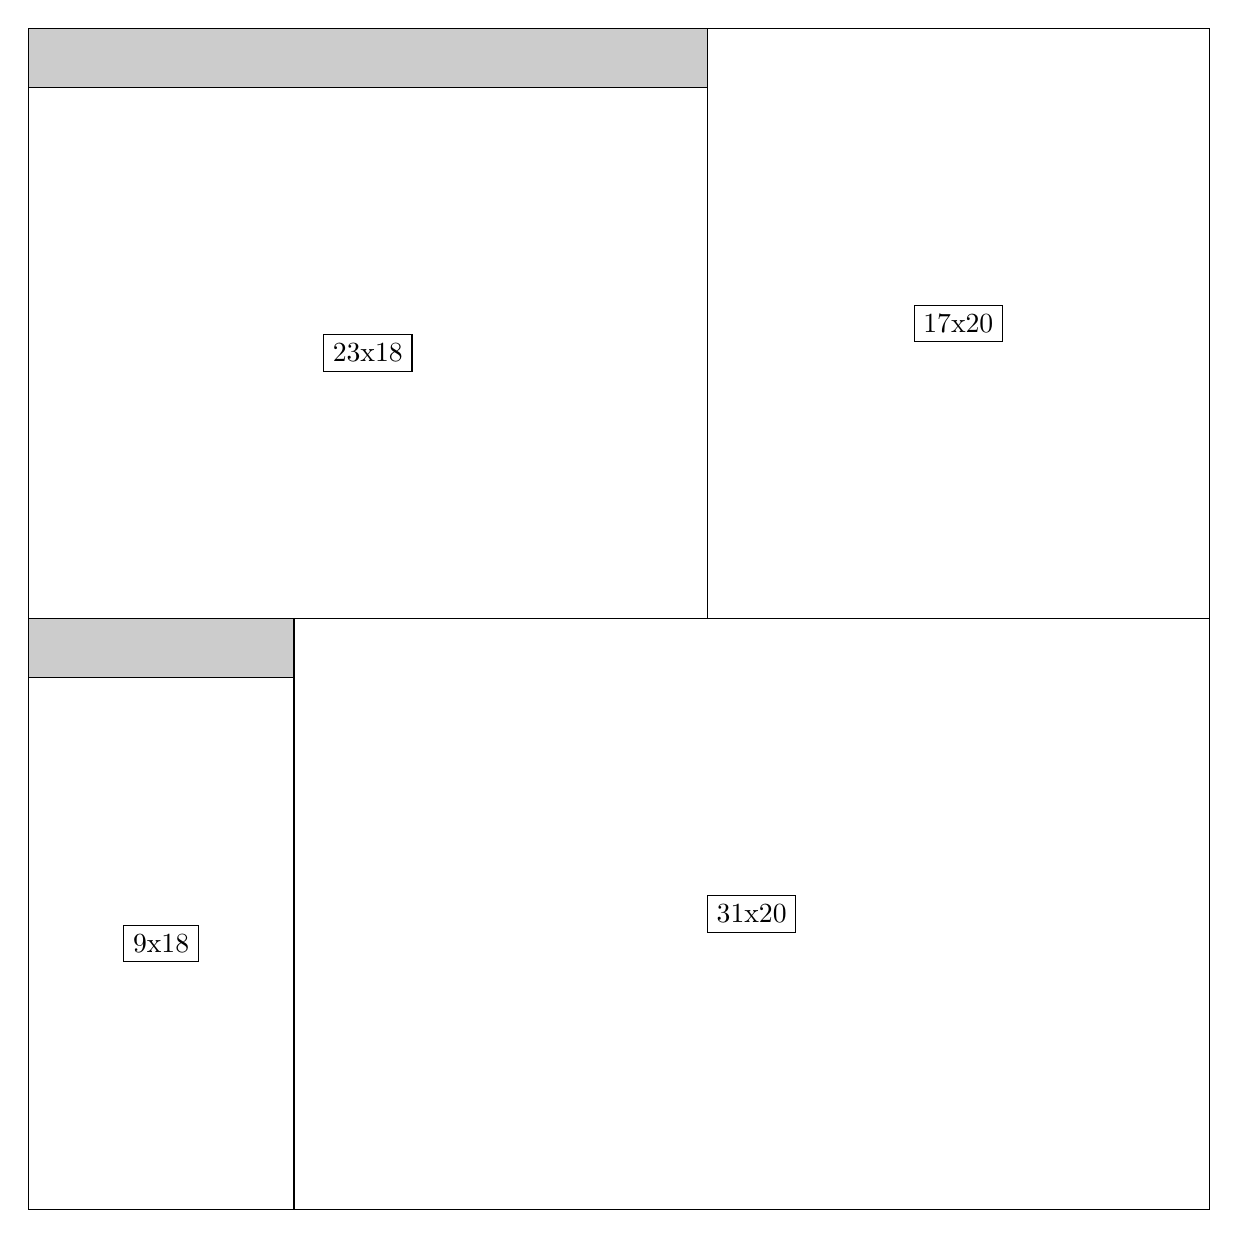
\begin{tikzpicture}[shorten >=1pt,scale=1.0,every node/.style={scale=1.0},->]
\tikzstyle{vertex}=[circle,fill=black!25,minimum size=14pt,inner sep=0pt]
\filldraw[fill=gray!40!white, draw=black] (0,0) rectangle (15.0,15.0);
\foreach \name/\x/\y/\w/\h in {31x20/3.375/0.0/11.625/7.5,9x18/0.0/0.0/3.375/6.75,17x20/8.625/7.5/6.375/7.5,23x18/0.0/7.5/8.625/6.75}
\filldraw[fill=white!40!white, draw=black] (\x,\y) rectangle node[draw] (\name) {\name} ++(\w,\h);
\end{tikzpicture}


w =31 , h =20 , x =9 , y =0 , v =620
\par
w =9 , h =18 , x =0 , y =0 , v =162
\par
w =17 , h =20 , x =23 , y =20 , v =340
\par
w =23 , h =18 , x =0 , y =20 , v =414
\par
\newpage


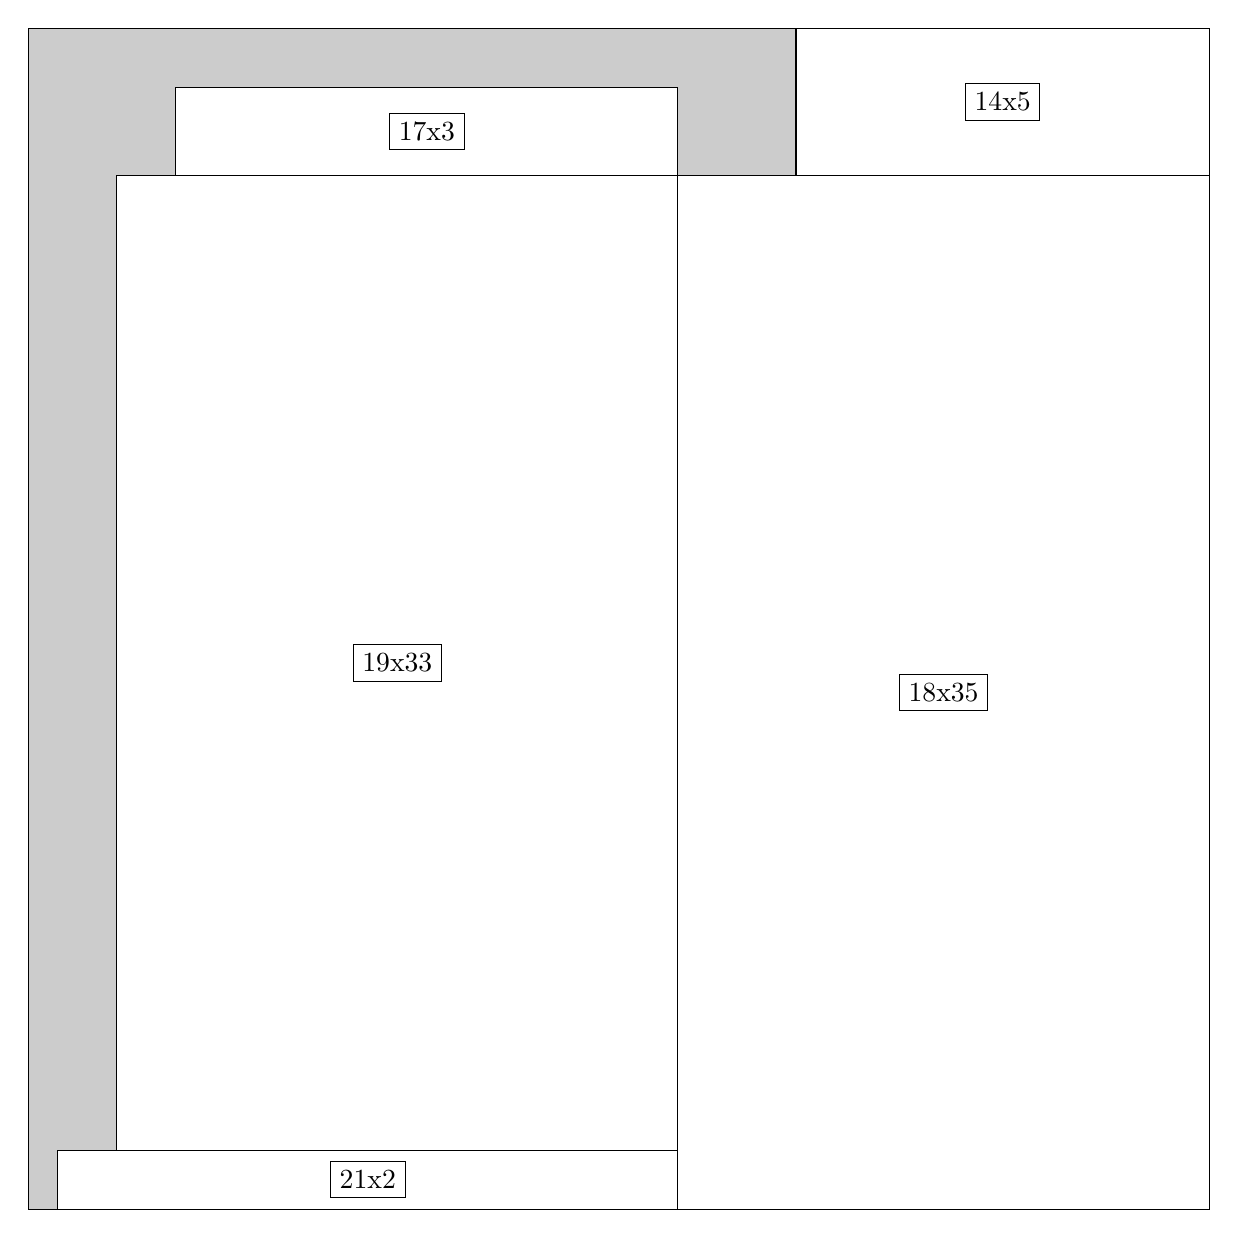
\begin{tikzpicture}[shorten >=1pt,scale=1.0,every node/.style={scale=1.0},->]
\tikzstyle{vertex}=[circle,fill=black!25,minimum size=14pt,inner sep=0pt]
\filldraw[fill=gray!40!white, draw=black] (0,0) rectangle (15.0,15.0);
\foreach \name/\x/\y/\w/\h in {18x35/8.25/0.0/6.75/13.125,14x5/9.75/13.125/5.25/1.875,21x2/0.375/0.0/7.875/0.75,19x33/1.125/0.75/7.125/12.375,17x3/1.875/13.125/6.375/1.125}
\filldraw[fill=white!40!white, draw=black] (\x,\y) rectangle node[draw] (\name) {\name} ++(\w,\h);
\end{tikzpicture}


w =18 , h =35 , x =22 , y =0 , v =630
\par
w =14 , h =5 , x =26 , y =35 , v =70
\par
w =21 , h =2 , x =1 , y =0 , v =42
\par
w =19 , h =33 , x =3 , y =2 , v =627
\par
w =17 , h =3 , x =5 , y =35 , v =51
\par
\newpage


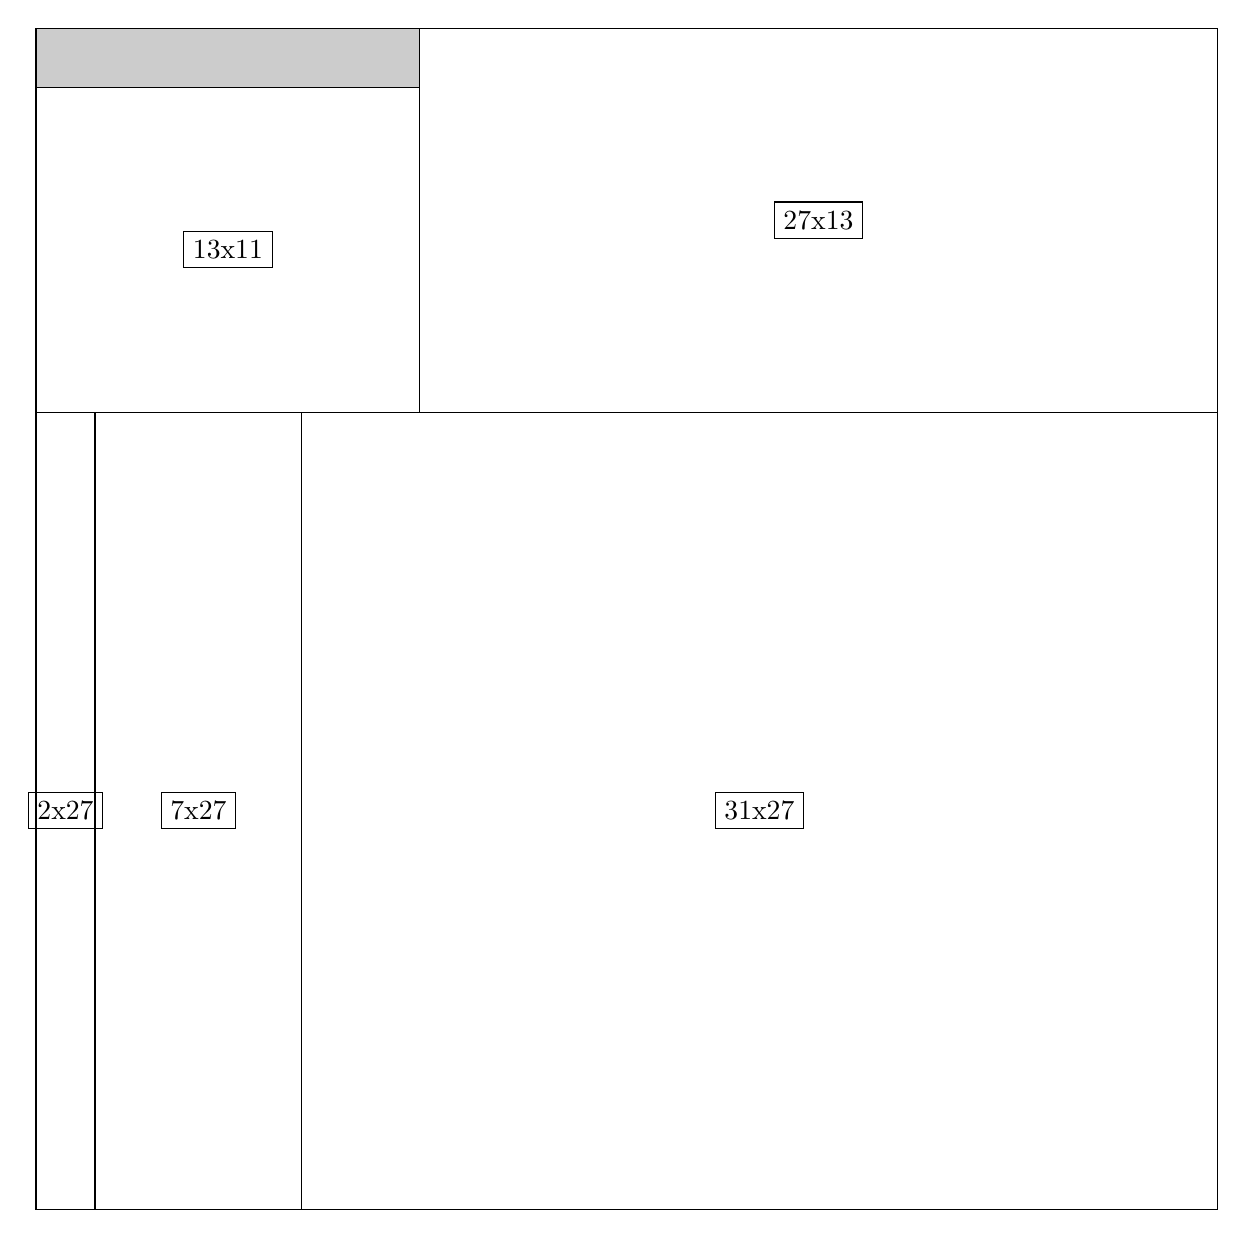
\begin{tikzpicture}[shorten >=1pt,scale=1.0,every node/.style={scale=1.0},->]
\tikzstyle{vertex}=[circle,fill=black!25,minimum size=14pt,inner sep=0pt]
\filldraw[fill=gray!40!white, draw=black] (0,0) rectangle (15.0,15.0);
\foreach \name/\x/\y/\w/\h in {31x27/3.375/0.0/11.625/10.125,7x27/0.75/0.0/2.625/10.125,2x27/0.0/0.0/0.75/10.125,27x13/4.875/10.125/10.125/4.875,13x11/0.0/10.125/4.875/4.125}
\filldraw[fill=white!40!white, draw=black] (\x,\y) rectangle node[draw] (\name) {\name} ++(\w,\h);
\end{tikzpicture}


w =31 , h =27 , x =9 , y =0 , v =837
\par
w =7 , h =27 , x =2 , y =0 , v =189
\par
w =2 , h =27 , x =0 , y =0 , v =54
\par
w =27 , h =13 , x =13 , y =27 , v =351
\par
w =13 , h =11 , x =0 , y =27 , v =143
\par
\newpage


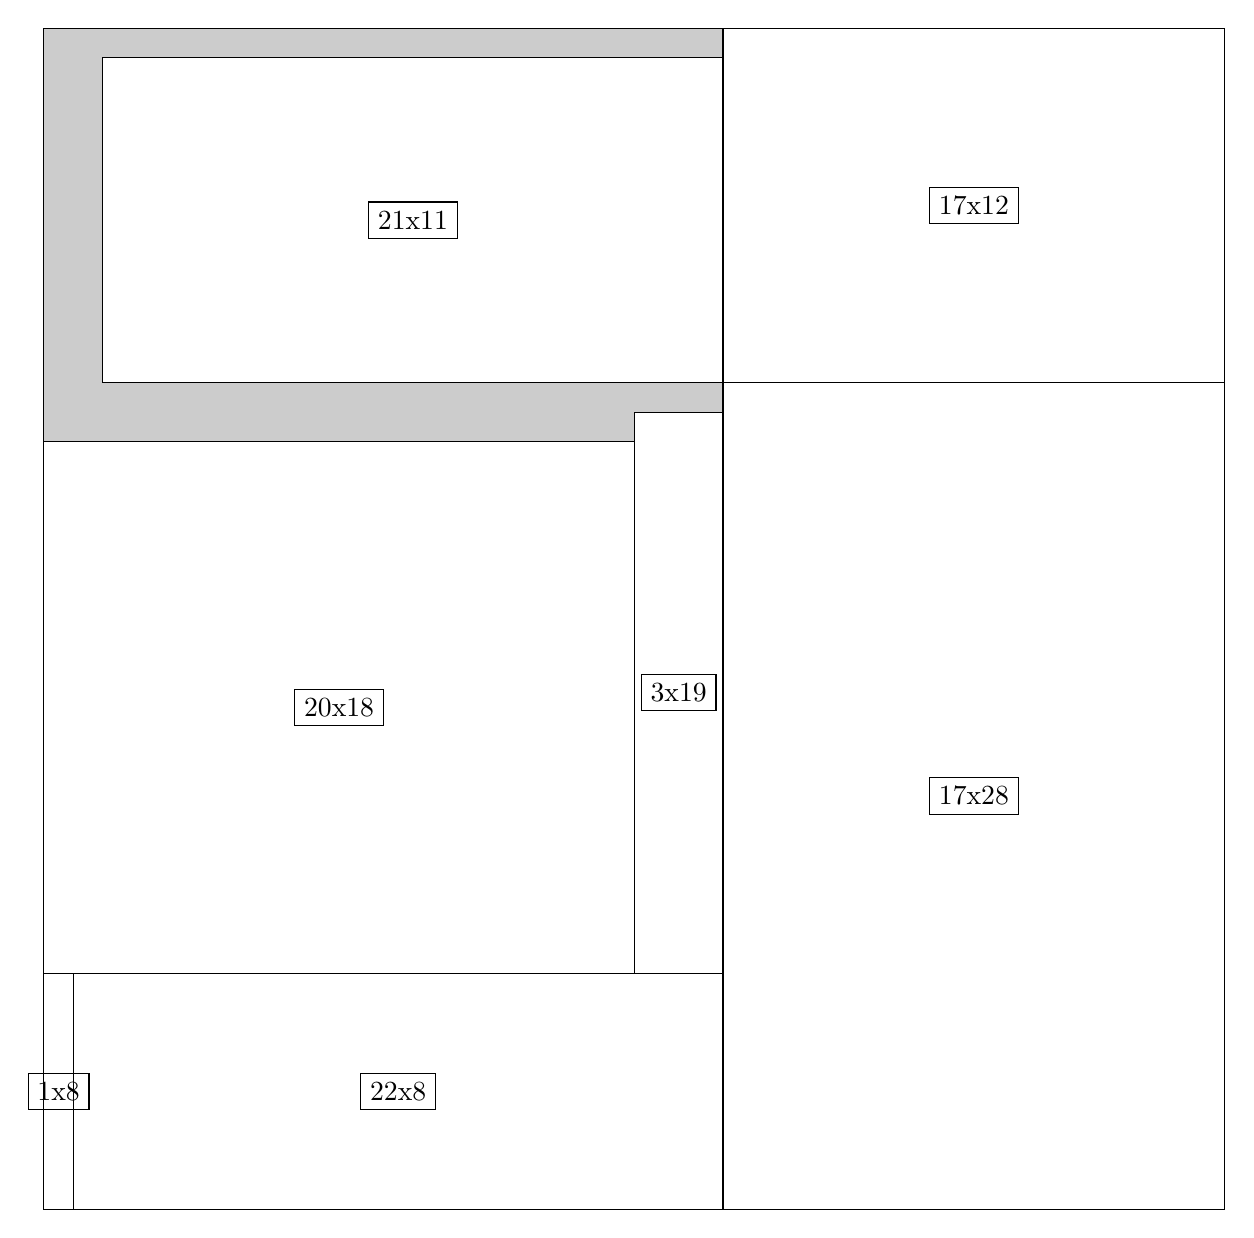
\begin{tikzpicture}[shorten >=1pt,scale=1.0,every node/.style={scale=1.0},->]
\tikzstyle{vertex}=[circle,fill=black!25,minimum size=14pt,inner sep=0pt]
\filldraw[fill=gray!40!white, draw=black] (0,0) rectangle (15.0,15.0);
\foreach \name/\x/\y/\w/\h in {17x28/8.625/0.0/6.375/10.5,22x8/0.375/0.0/8.25/3.0,1x8/0.0/0.0/0.375/3.0,3x19/7.5/3.0/1.125/7.125,20x18/0.0/3.0/7.5/6.75,17x12/8.625/10.5/6.375/4.5,21x11/0.75/10.5/7.875/4.125}
\filldraw[fill=white!40!white, draw=black] (\x,\y) rectangle node[draw] (\name) {\name} ++(\w,\h);
\end{tikzpicture}


w =17 , h =28 , x =23 , y =0 , v =476
\par
w =22 , h =8 , x =1 , y =0 , v =176
\par
w =1 , h =8 , x =0 , y =0 , v =8
\par
w =3 , h =19 , x =20 , y =8 , v =57
\par
w =20 , h =18 , x =0 , y =8 , v =360
\par
w =17 , h =12 , x =23 , y =28 , v =204
\par
w =21 , h =11 , x =2 , y =28 , v =231
\par
\newpage


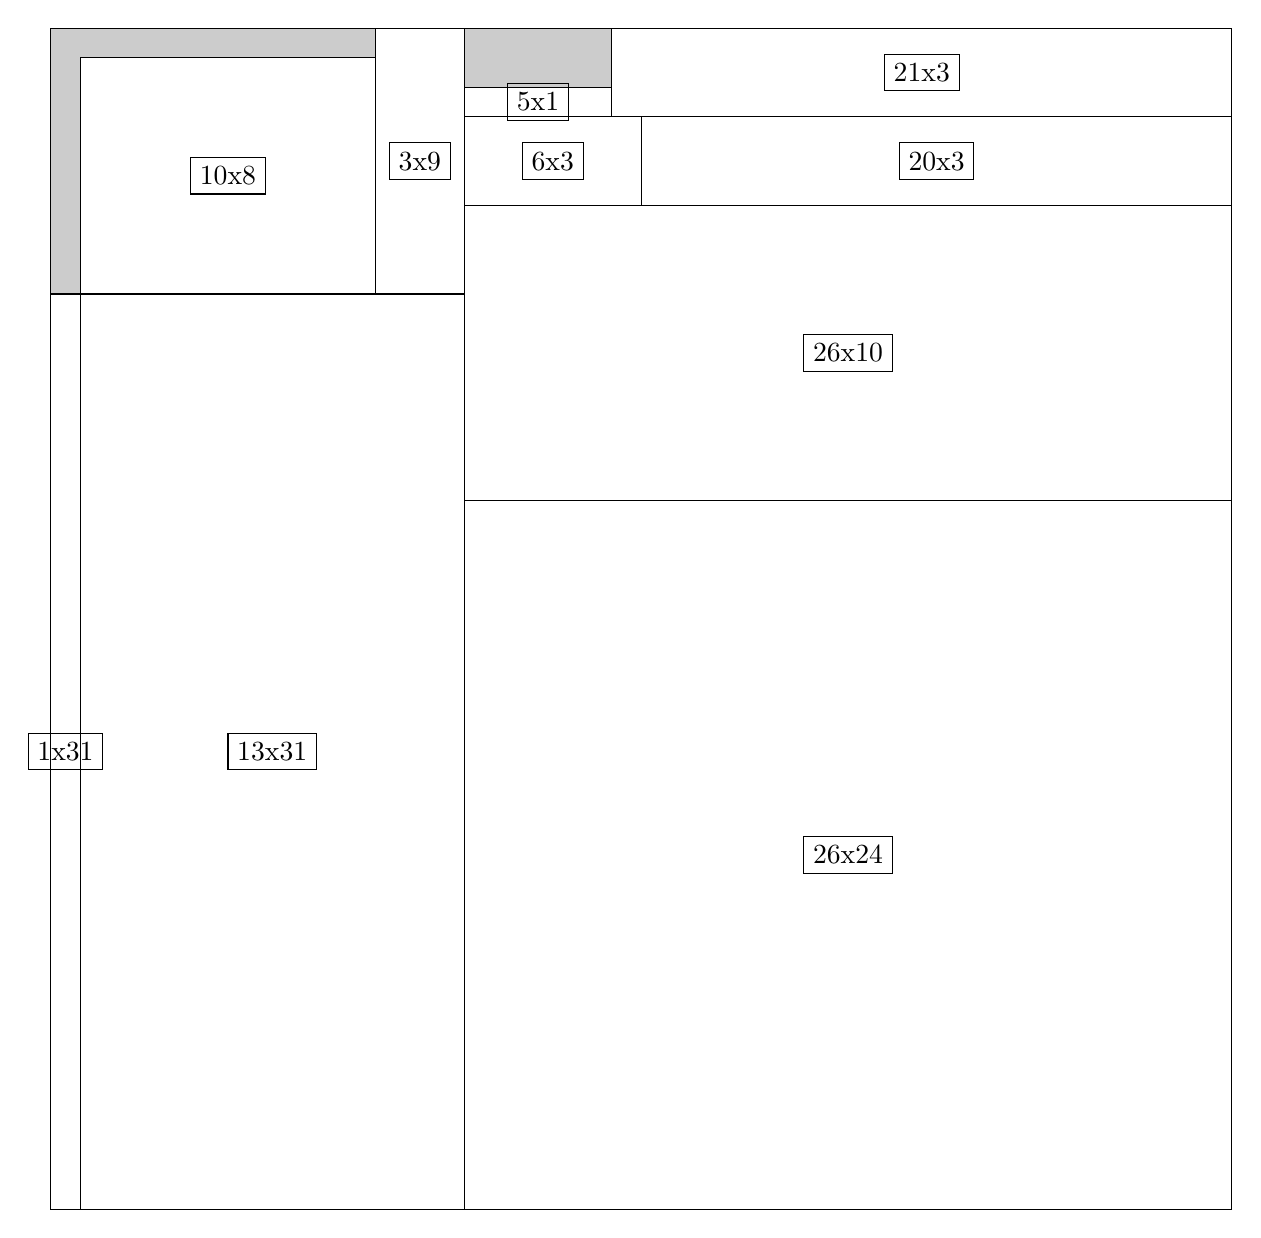
\begin{tikzpicture}[shorten >=1pt,scale=1.0,every node/.style={scale=1.0},->]
\tikzstyle{vertex}=[circle,fill=black!25,minimum size=14pt,inner sep=0pt]
\filldraw[fill=gray!40!white, draw=black] (0,0) rectangle (15.0,15.0);
\foreach \name/\x/\y/\w/\h in {26x24/5.25/0.0/9.75/9.0,26x10/5.25/9.0/9.75/3.75,20x3/7.5/12.75/7.5/1.125,6x3/5.25/12.75/2.25/1.125,21x3/7.125/13.875/7.875/1.125,5x1/5.25/13.875/1.875/0.375,13x31/0.375/0.0/4.875/11.625,1x31/0.0/0.0/0.375/11.625,3x9/4.125/11.625/1.125/3.375,10x8/0.375/11.625/3.75/3.0}
\filldraw[fill=white!40!white, draw=black] (\x,\y) rectangle node[draw] (\name) {\name} ++(\w,\h);
\end{tikzpicture}


w =26 , h =24 , x =14 , y =0 , v =624
\par
w =26 , h =10 , x =14 , y =24 , v =260
\par
w =20 , h =3 , x =20 , y =34 , v =60
\par
w =6 , h =3 , x =14 , y =34 , v =18
\par
w =21 , h =3 , x =19 , y =37 , v =63
\par
w =5 , h =1 , x =14 , y =37 , v =5
\par
w =13 , h =31 , x =1 , y =0 , v =403
\par
w =1 , h =31 , x =0 , y =0 , v =31
\par
w =3 , h =9 , x =11 , y =31 , v =27
\par
w =10 , h =8 , x =1 , y =31 , v =80
\par
\newpage


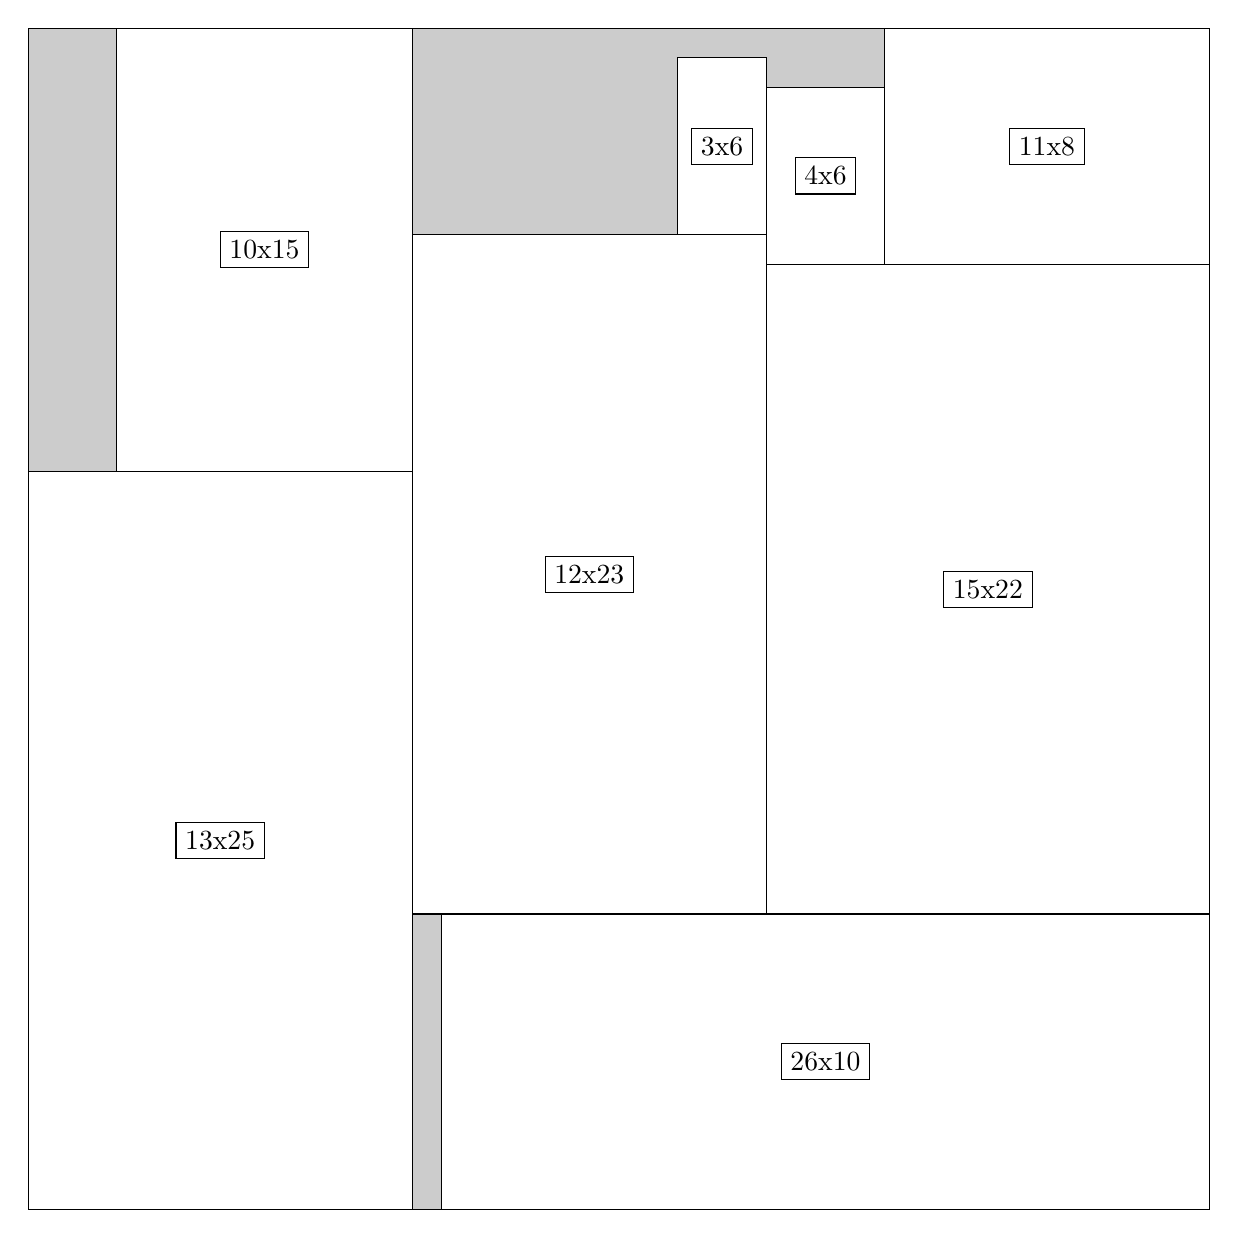
\begin{tikzpicture}[shorten >=1pt,scale=1.0,every node/.style={scale=1.0},->]
\tikzstyle{vertex}=[circle,fill=black!25,minimum size=14pt,inner sep=0pt]
\filldraw[fill=gray!40!white, draw=black] (0,0) rectangle (15.0,15.0);
\foreach \name/\x/\y/\w/\h in {26x10/5.25/0.0/9.75/3.75,15x22/9.375/3.75/5.625/8.25,11x8/10.875/12.0/4.125/3.0,4x6/9.375/12.0/1.5/2.25,12x23/4.875/3.75/4.5/8.625,3x6/8.25/12.375/1.125/2.25,13x25/0.0/0.0/4.875/9.375,10x15/1.125/9.375/3.75/5.625}
\filldraw[fill=white!40!white, draw=black] (\x,\y) rectangle node[draw] (\name) {\name} ++(\w,\h);
\end{tikzpicture}


w =26 , h =10 , x =14 , y =0 , v =260
\par
w =15 , h =22 , x =25 , y =10 , v =330
\par
w =11 , h =8 , x =29 , y =32 , v =88
\par
w =4 , h =6 , x =25 , y =32 , v =24
\par
w =12 , h =23 , x =13 , y =10 , v =276
\par
w =3 , h =6 , x =22 , y =33 , v =18
\par
w =13 , h =25 , x =0 , y =0 , v =325
\par
w =10 , h =15 , x =3 , y =25 , v =150
\par
\newpage


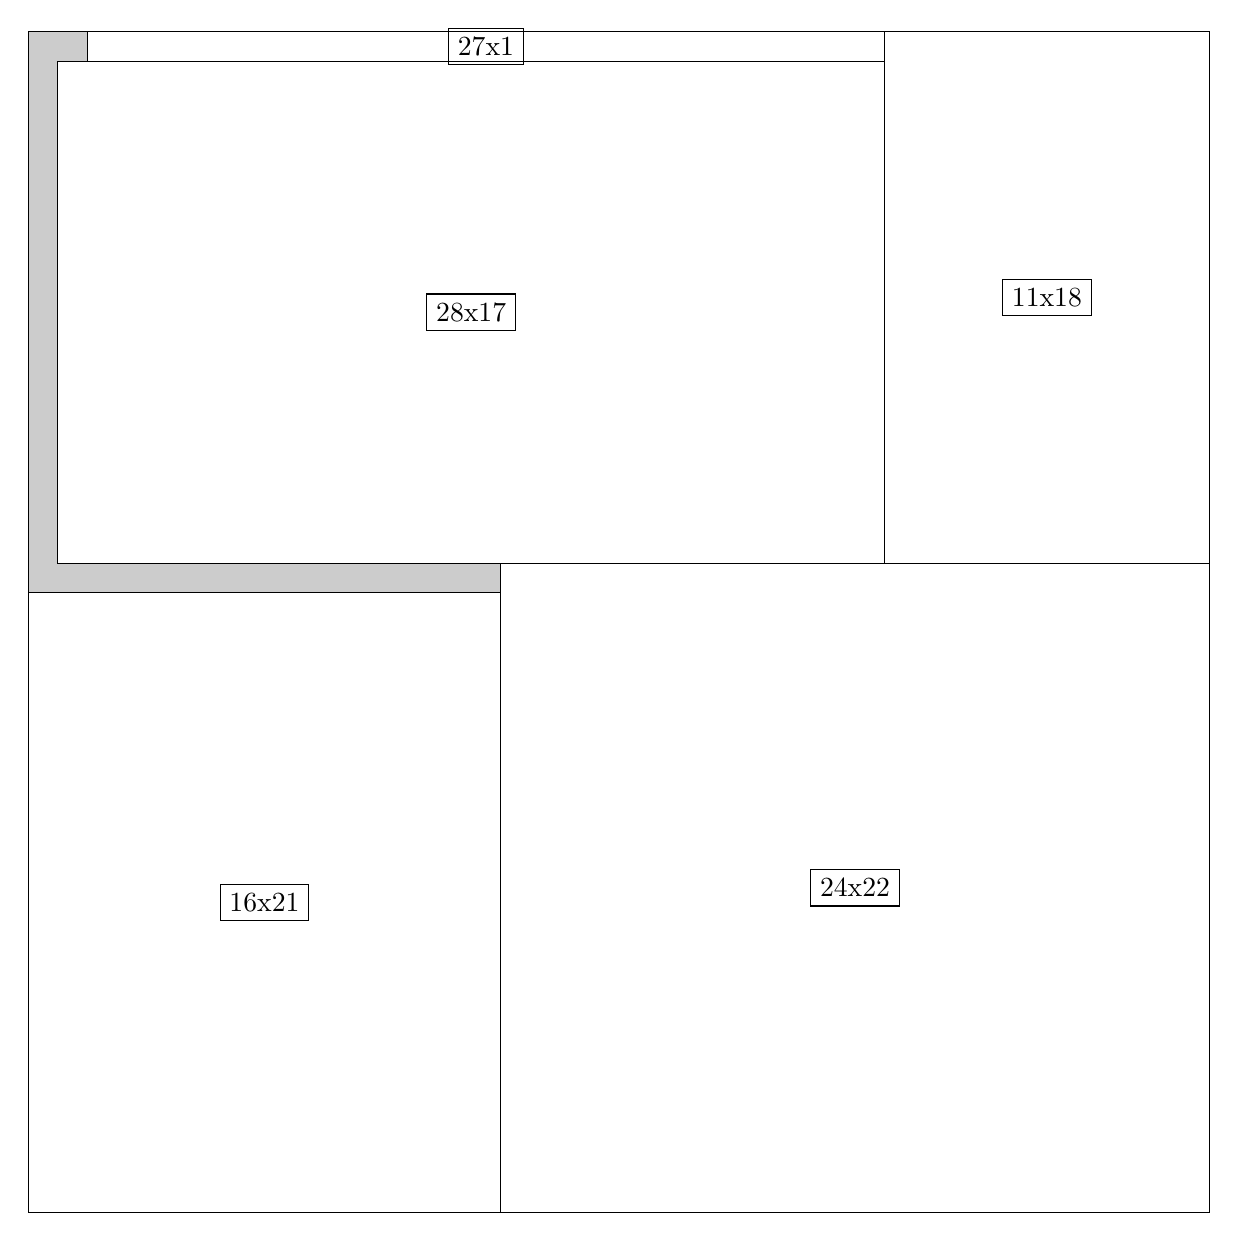
\begin{tikzpicture}[shorten >=1pt,scale=1.0,every node/.style={scale=1.0},->]
\tikzstyle{vertex}=[circle,fill=black!25,minimum size=14pt,inner sep=0pt]
\filldraw[fill=gray!40!white, draw=black] (0,0) rectangle (15.0,15.0);
\foreach \name/\x/\y/\w/\h in {24x22/6.0/0.0/9.0/8.25,16x21/0.0/0.0/6.0/7.875,11x18/10.875/8.25/4.125/6.75,28x17/0.375/8.25/10.5/6.375,27x1/0.75/14.625/10.125/0.375}
\filldraw[fill=white!40!white, draw=black] (\x,\y) rectangle node[draw] (\name) {\name} ++(\w,\h);
\end{tikzpicture}


w =24 , h =22 , x =16 , y =0 , v =528
\par
w =16 , h =21 , x =0 , y =0 , v =336
\par
w =11 , h =18 , x =29 , y =22 , v =198
\par
w =28 , h =17 , x =1 , y =22 , v =476
\par
w =27 , h =1 , x =2 , y =39 , v =27
\par
\newpage


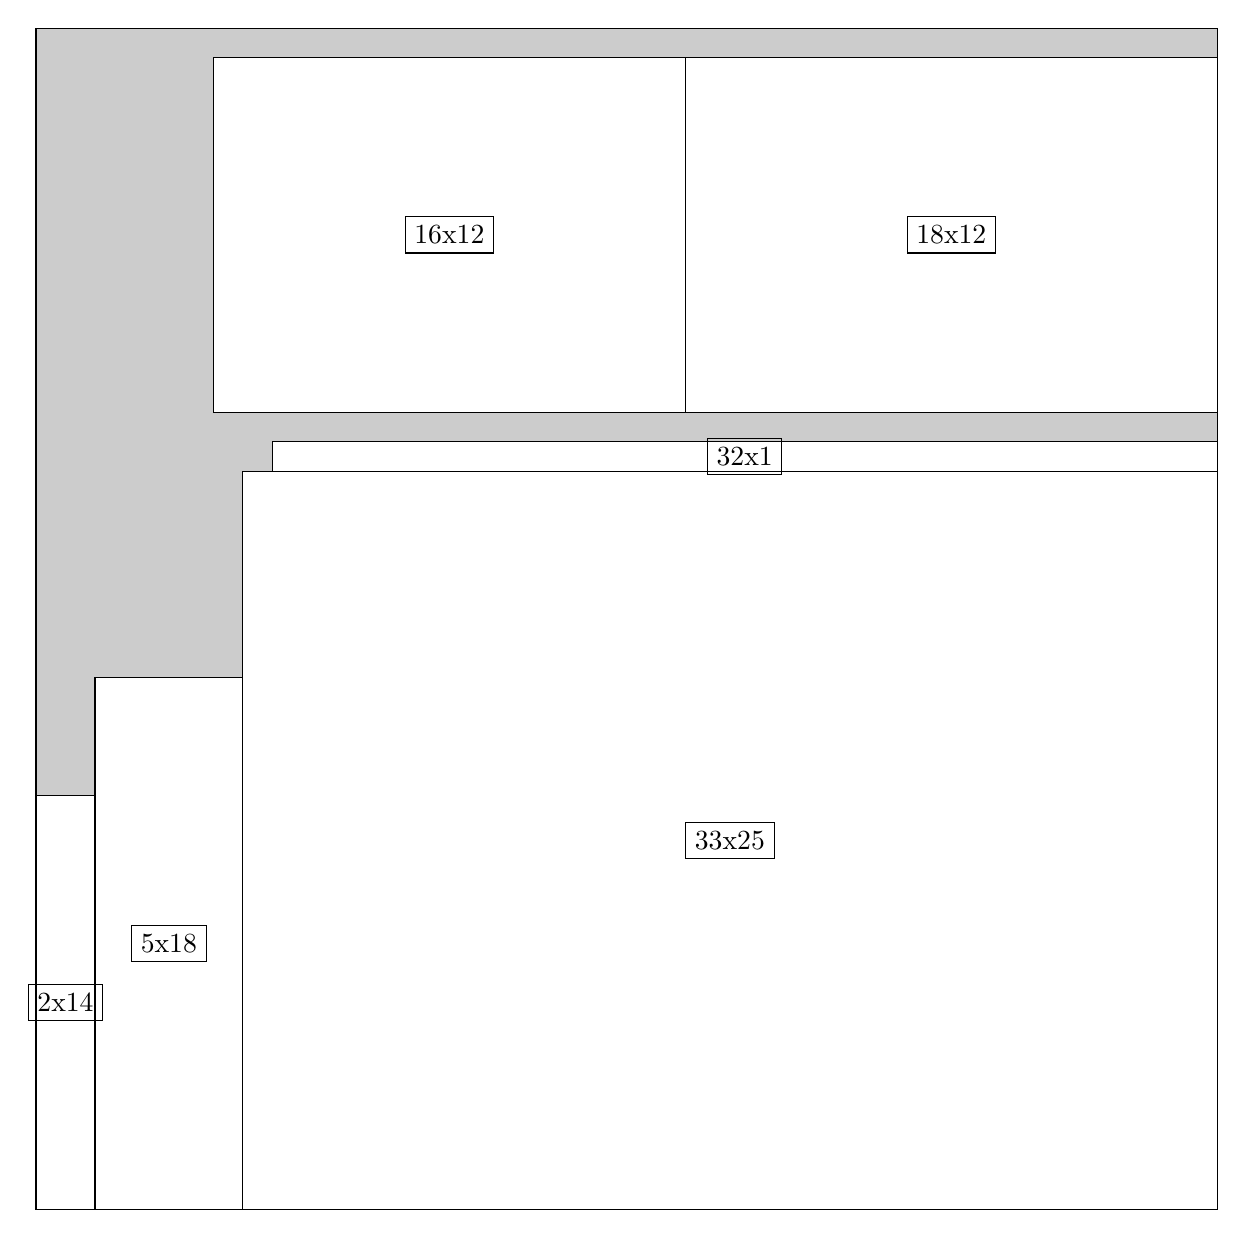
\begin{tikzpicture}[shorten >=1pt,scale=1.0,every node/.style={scale=1.0},->]
\tikzstyle{vertex}=[circle,fill=black!25,minimum size=14pt,inner sep=0pt]
\filldraw[fill=gray!40!white, draw=black] (0,0) rectangle (15.0,15.0);
\foreach \name/\x/\y/\w/\h in {33x25/2.625/0.0/12.375/9.375,32x1/3.0/9.375/12.0/0.375,5x18/0.75/0.0/1.875/6.75,2x14/0.0/0.0/0.75/5.25,18x12/8.25/10.125/6.75/4.5,16x12/2.25/10.125/6.0/4.5}
\filldraw[fill=white!40!white, draw=black] (\x,\y) rectangle node[draw] (\name) {\name} ++(\w,\h);
\end{tikzpicture}


w =33 , h =25 , x =7 , y =0 , v =825
\par
w =32 , h =1 , x =8 , y =25 , v =32
\par
w =5 , h =18 , x =2 , y =0 , v =90
\par
w =2 , h =14 , x =0 , y =0 , v =28
\par
w =18 , h =12 , x =22 , y =27 , v =216
\par
w =16 , h =12 , x =6 , y =27 , v =192
\par
\newpage


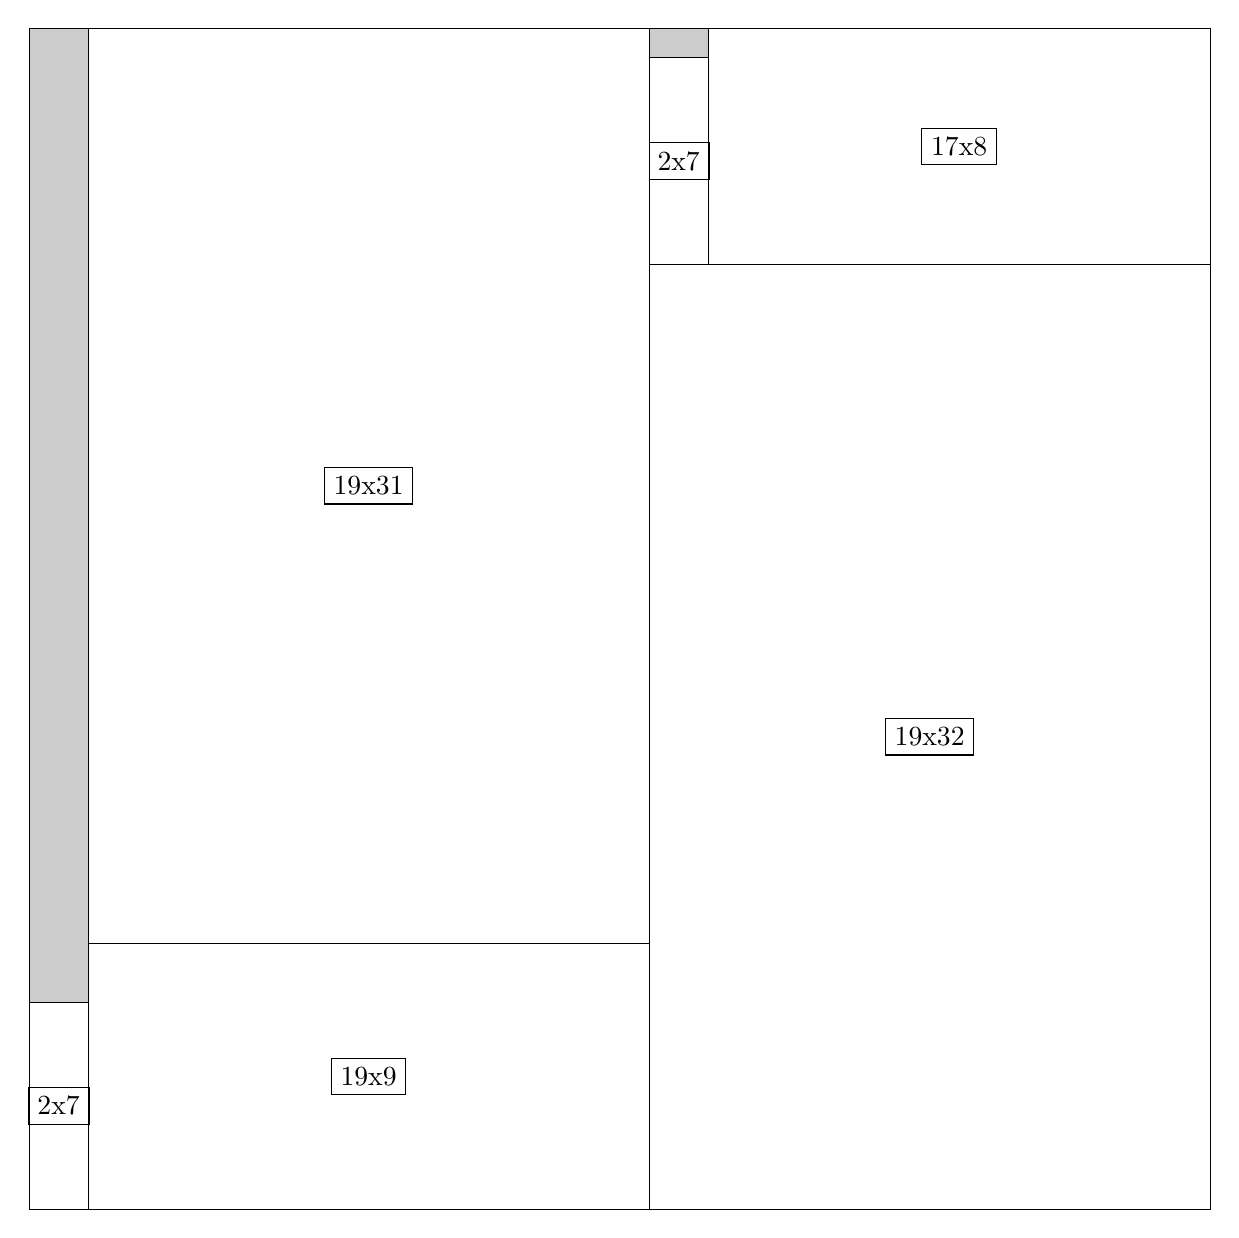
\begin{tikzpicture}[shorten >=1pt,scale=1.0,every node/.style={scale=1.0},->]
\tikzstyle{vertex}=[circle,fill=black!25,minimum size=14pt,inner sep=0pt]
\filldraw[fill=gray!40!white, draw=black] (0,0) rectangle (15.0,15.0);
\foreach \name/\x/\y/\w/\h in {19x32/7.875/0.0/7.125/12.0,17x8/8.625/12.0/6.375/3.0,2x7/7.875/12.0/0.75/2.625,19x9/0.75/0.0/7.125/3.375,2x7/0.0/0.0/0.75/2.625,19x31/0.75/3.375/7.125/11.625}
\filldraw[fill=white!40!white, draw=black] (\x,\y) rectangle node[draw] (\name) {\name} ++(\w,\h);
\end{tikzpicture}


w =19 , h =32 , x =21 , y =0 , v =608
\par
w =17 , h =8 , x =23 , y =32 , v =136
\par
w =2 , h =7 , x =21 , y =32 , v =14
\par
w =19 , h =9 , x =2 , y =0 , v =171
\par
w =2 , h =7 , x =0 , y =0 , v =14
\par
w =19 , h =31 , x =2 , y =9 , v =589
\par
\newpage


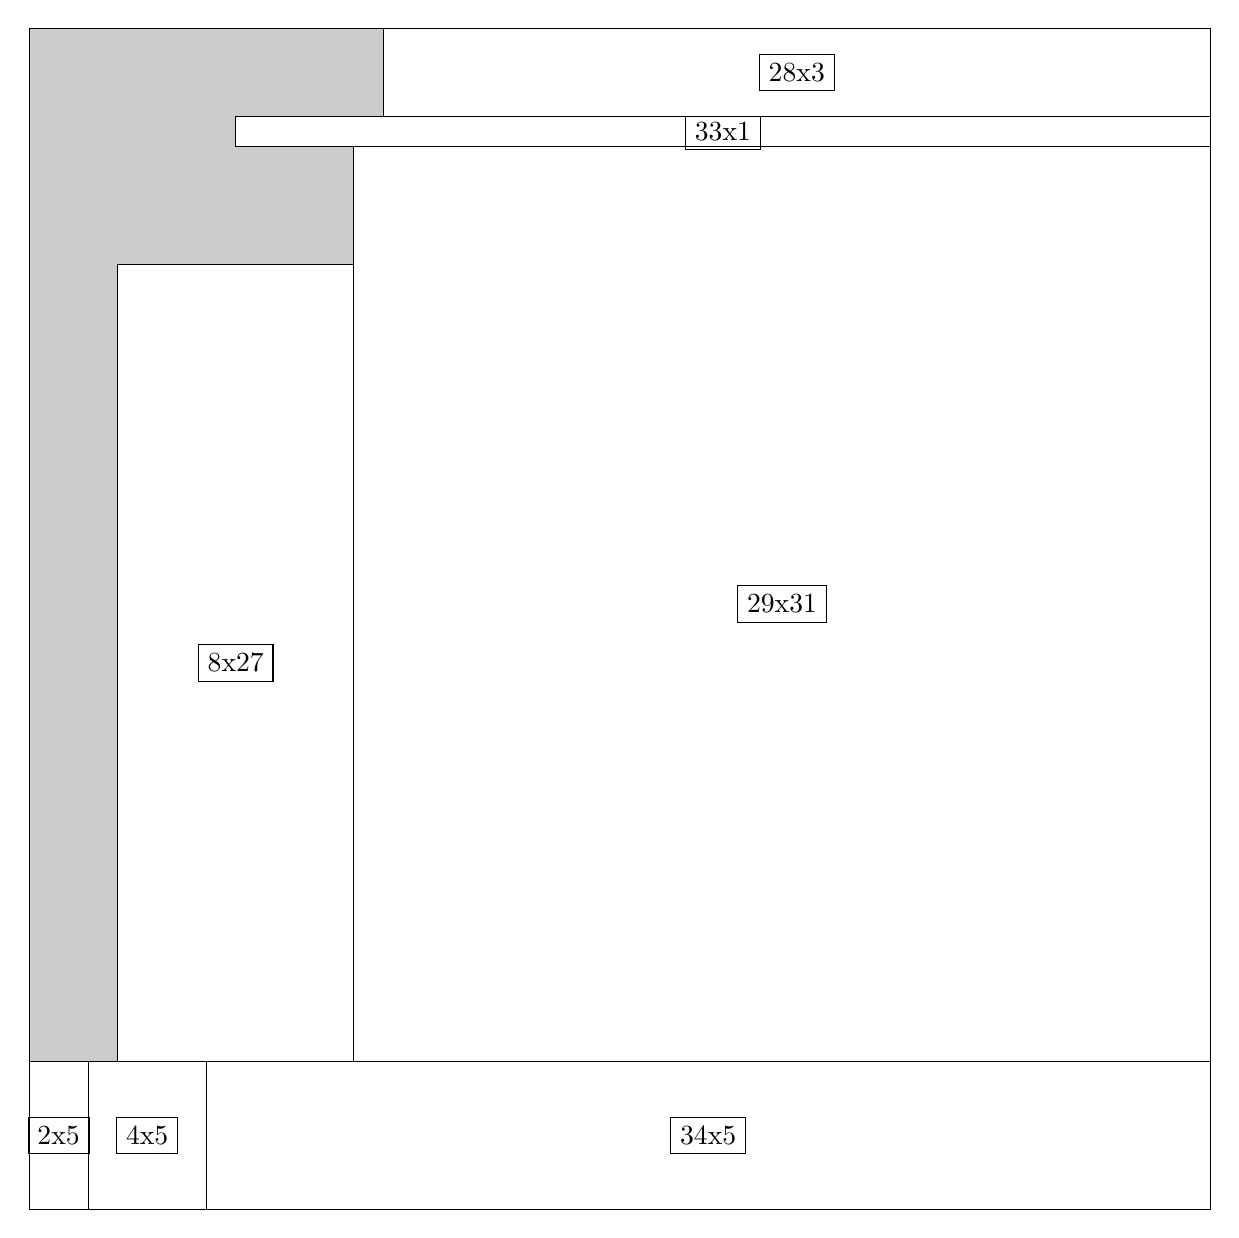
\begin{tikzpicture}[shorten >=1pt,scale=1.0,every node/.style={scale=1.0},->]
\tikzstyle{vertex}=[circle,fill=black!25,minimum size=14pt,inner sep=0pt]
\filldraw[fill=gray!40!white, draw=black] (0,0) rectangle (15.0,15.0);
\foreach \name/\x/\y/\w/\h in {34x5/2.25/0.0/12.75/1.875,4x5/0.75/0.0/1.5/1.875,2x5/0.0/0.0/0.75/1.875,29x31/4.125/1.875/10.875/11.625,8x27/1.125/1.875/3.0/10.125,33x1/2.625/13.5/12.375/0.375,28x3/4.5/13.875/10.5/1.125}
\filldraw[fill=white!40!white, draw=black] (\x,\y) rectangle node[draw] (\name) {\name} ++(\w,\h);
\end{tikzpicture}


w =34 , h =5 , x =6 , y =0 , v =170
\par
w =4 , h =5 , x =2 , y =0 , v =20
\par
w =2 , h =5 , x =0 , y =0 , v =10
\par
w =29 , h =31 , x =11 , y =5 , v =899
\par
w =8 , h =27 , x =3 , y =5 , v =216
\par
w =33 , h =1 , x =7 , y =36 , v =33
\par
w =28 , h =3 , x =12 , y =37 , v =84
\par
\newpage


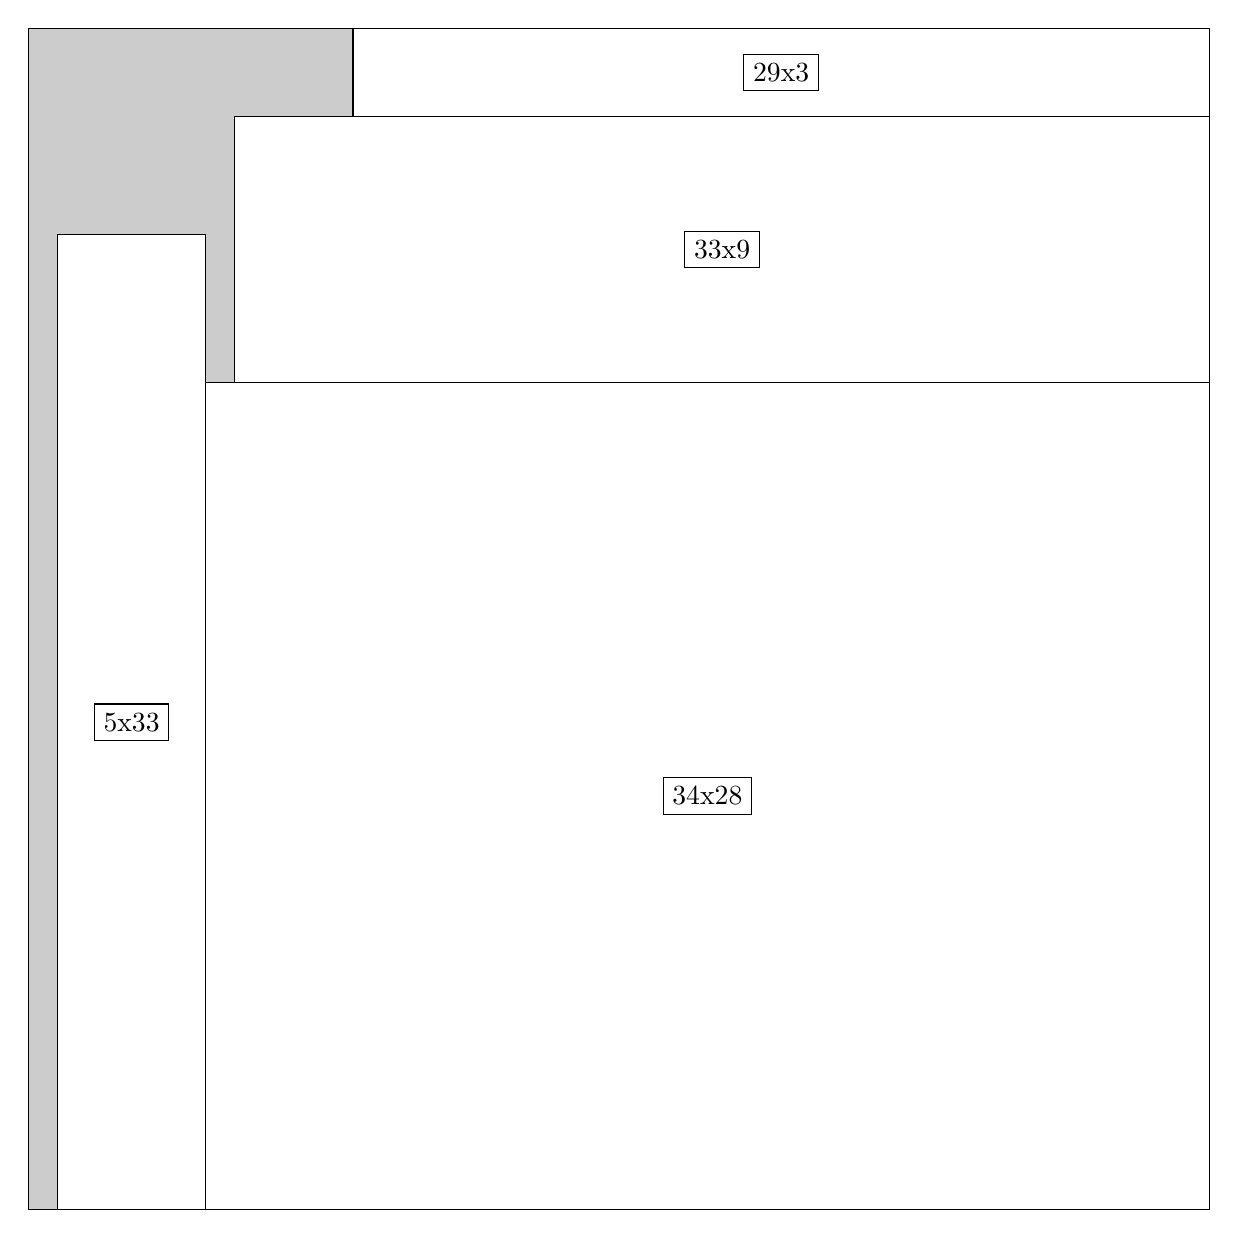
\begin{tikzpicture}[shorten >=1pt,scale=1.0,every node/.style={scale=1.0},->]
\tikzstyle{vertex}=[circle,fill=black!25,minimum size=14pt,inner sep=0pt]
\filldraw[fill=gray!40!white, draw=black] (0,0) rectangle (15.0,15.0);
\foreach \name/\x/\y/\w/\h in {34x28/2.25/0.0/12.75/10.5,33x9/2.625/10.5/12.375/3.375,29x3/4.125/13.875/10.875/1.125,5x33/0.375/0.0/1.875/12.375}
\filldraw[fill=white!40!white, draw=black] (\x,\y) rectangle node[draw] (\name) {\name} ++(\w,\h);
\end{tikzpicture}


w =34 , h =28 , x =6 , y =0 , v =952
\par
w =33 , h =9 , x =7 , y =28 , v =297
\par
w =29 , h =3 , x =11 , y =37 , v =87
\par
w =5 , h =33 , x =1 , y =0 , v =165
\par
\newpage


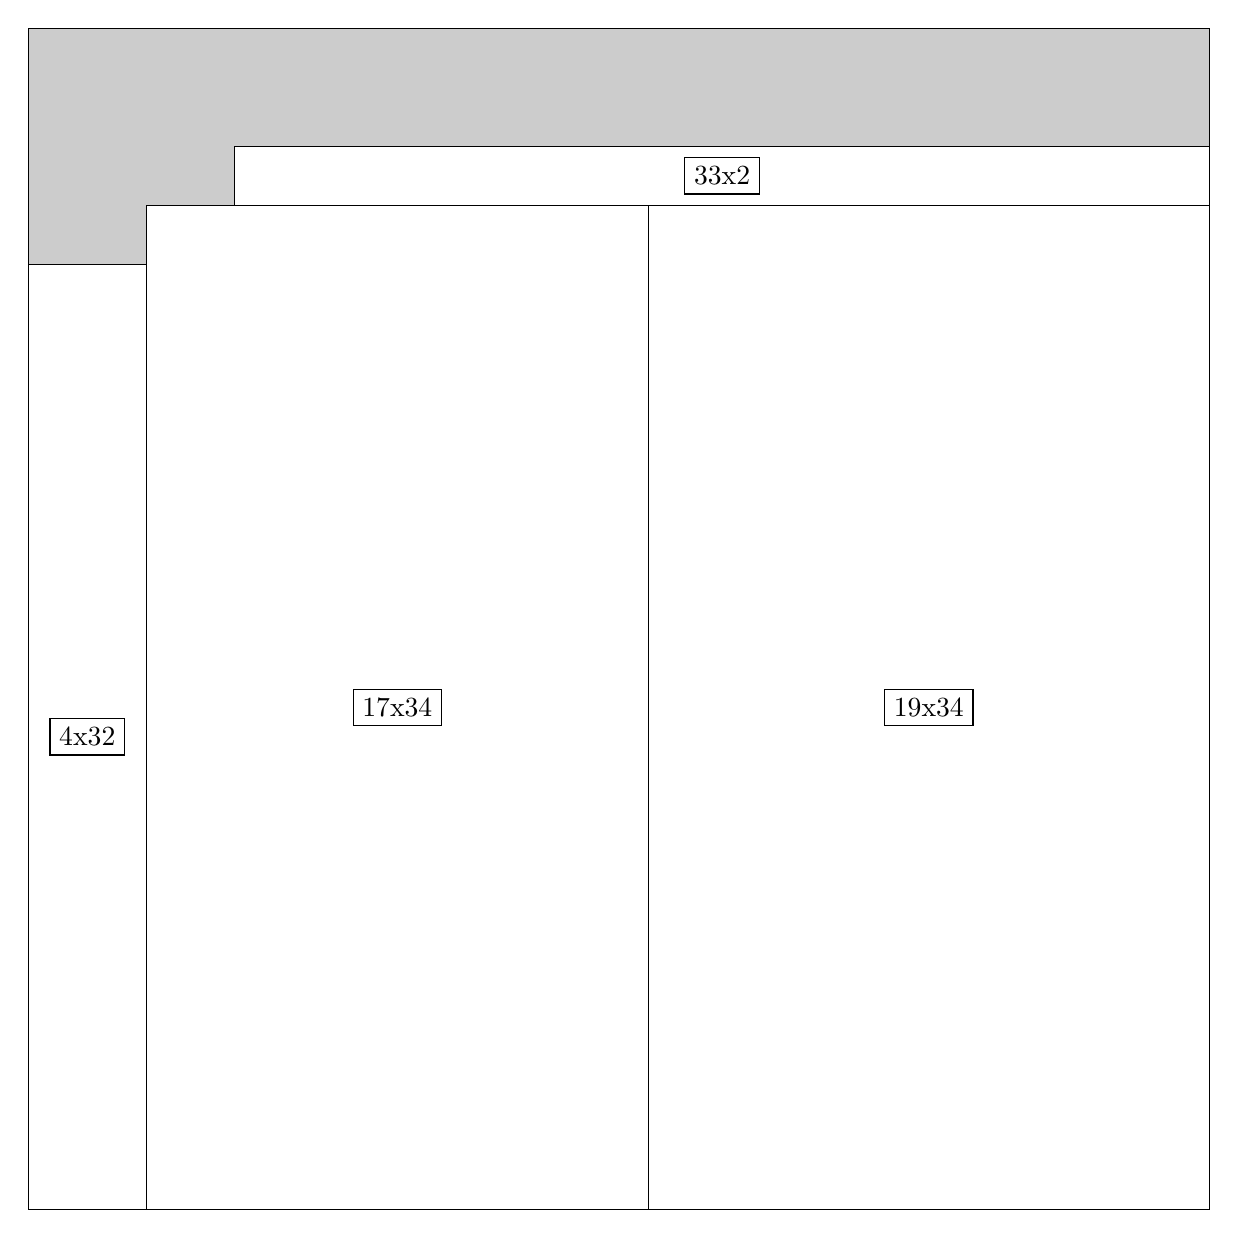
\begin{tikzpicture}[shorten >=1pt,scale=1.0,every node/.style={scale=1.0},->]
\tikzstyle{vertex}=[circle,fill=black!25,minimum size=14pt,inner sep=0pt]
\filldraw[fill=gray!40!white, draw=black] (0,0) rectangle (15.0,15.0);
\foreach \name/\x/\y/\w/\h in {19x34/7.875/0.0/7.125/12.75,17x34/1.5/0.0/6.375/12.75,4x32/0.0/0.0/1.5/12.0,33x2/2.625/12.75/12.375/0.75}
\filldraw[fill=white!40!white, draw=black] (\x,\y) rectangle node[draw] (\name) {\name} ++(\w,\h);
\end{tikzpicture}


w =19 , h =34 , x =21 , y =0 , v =646
\par
w =17 , h =34 , x =4 , y =0 , v =578
\par
w =4 , h =32 , x =0 , y =0 , v =128
\par
w =33 , h =2 , x =7 , y =34 , v =66
\par
\newpage


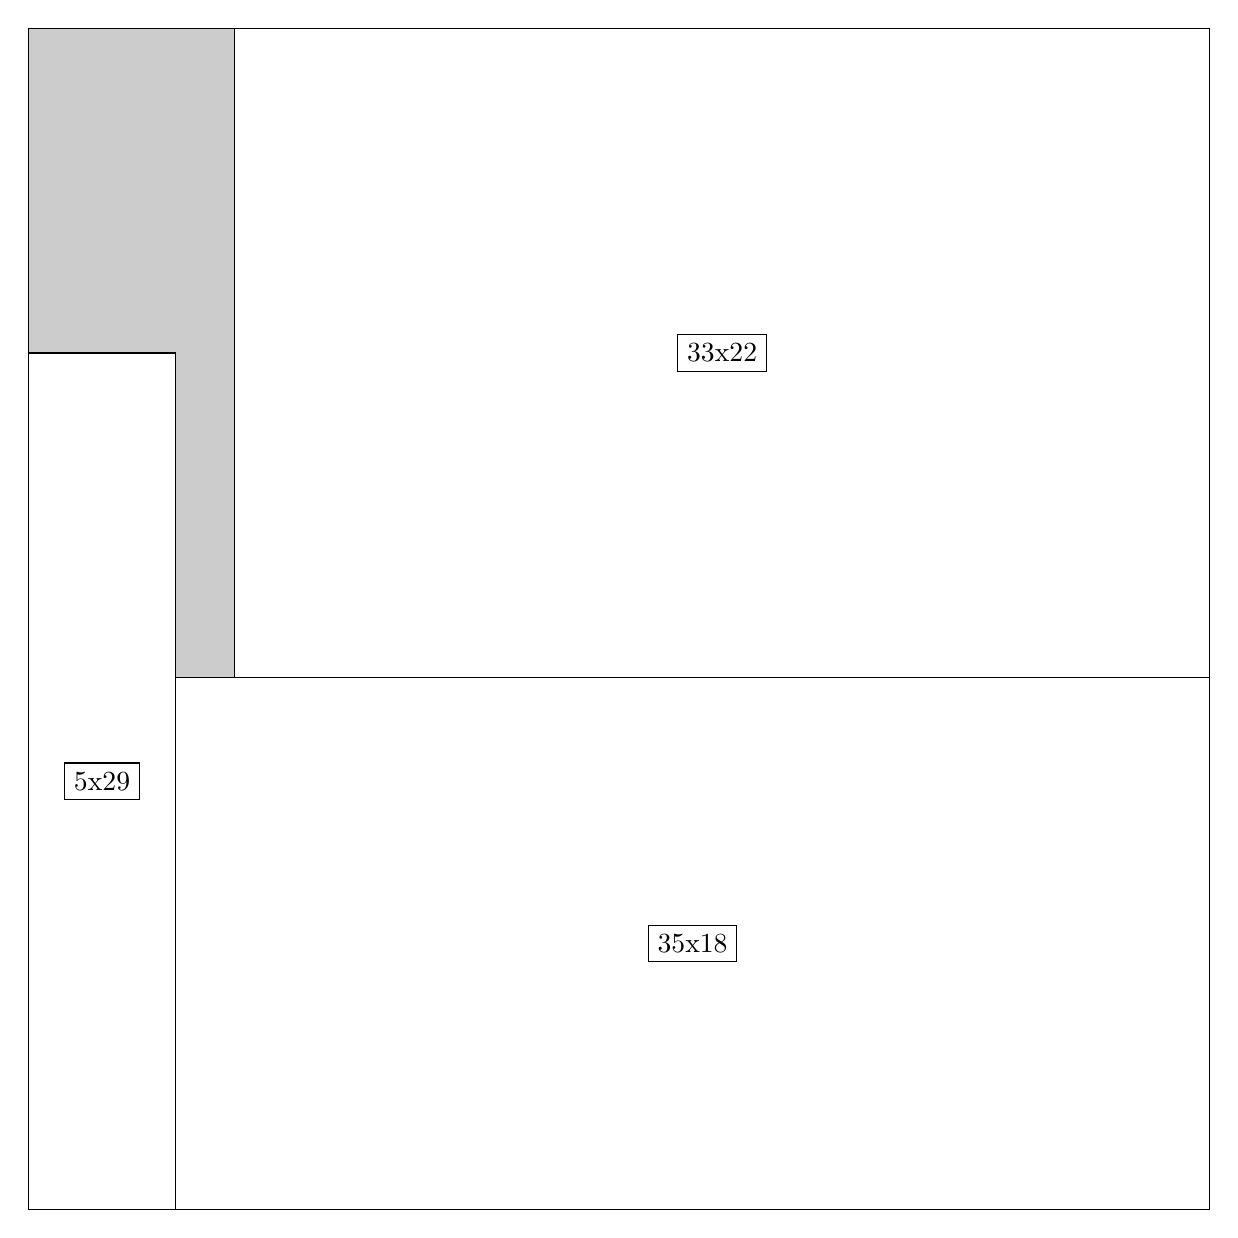
\begin{tikzpicture}[shorten >=1pt,scale=1.0,every node/.style={scale=1.0},->]
\tikzstyle{vertex}=[circle,fill=black!25,minimum size=14pt,inner sep=0pt]
\filldraw[fill=gray!40!white, draw=black] (0,0) rectangle (15.0,15.0);
\foreach \name/\x/\y/\w/\h in {35x18/1.875/0.0/13.125/6.75,33x22/2.625/6.75/12.375/8.25,5x29/0.0/0.0/1.875/10.875}
\filldraw[fill=white!40!white, draw=black] (\x,\y) rectangle node[draw] (\name) {\name} ++(\w,\h);
\end{tikzpicture}


w =35 , h =18 , x =5 , y =0 , v =630
\par
w =33 , h =22 , x =7 , y =18 , v =726
\par
w =5 , h =29 , x =0 , y =0 , v =145
\par
\newpage


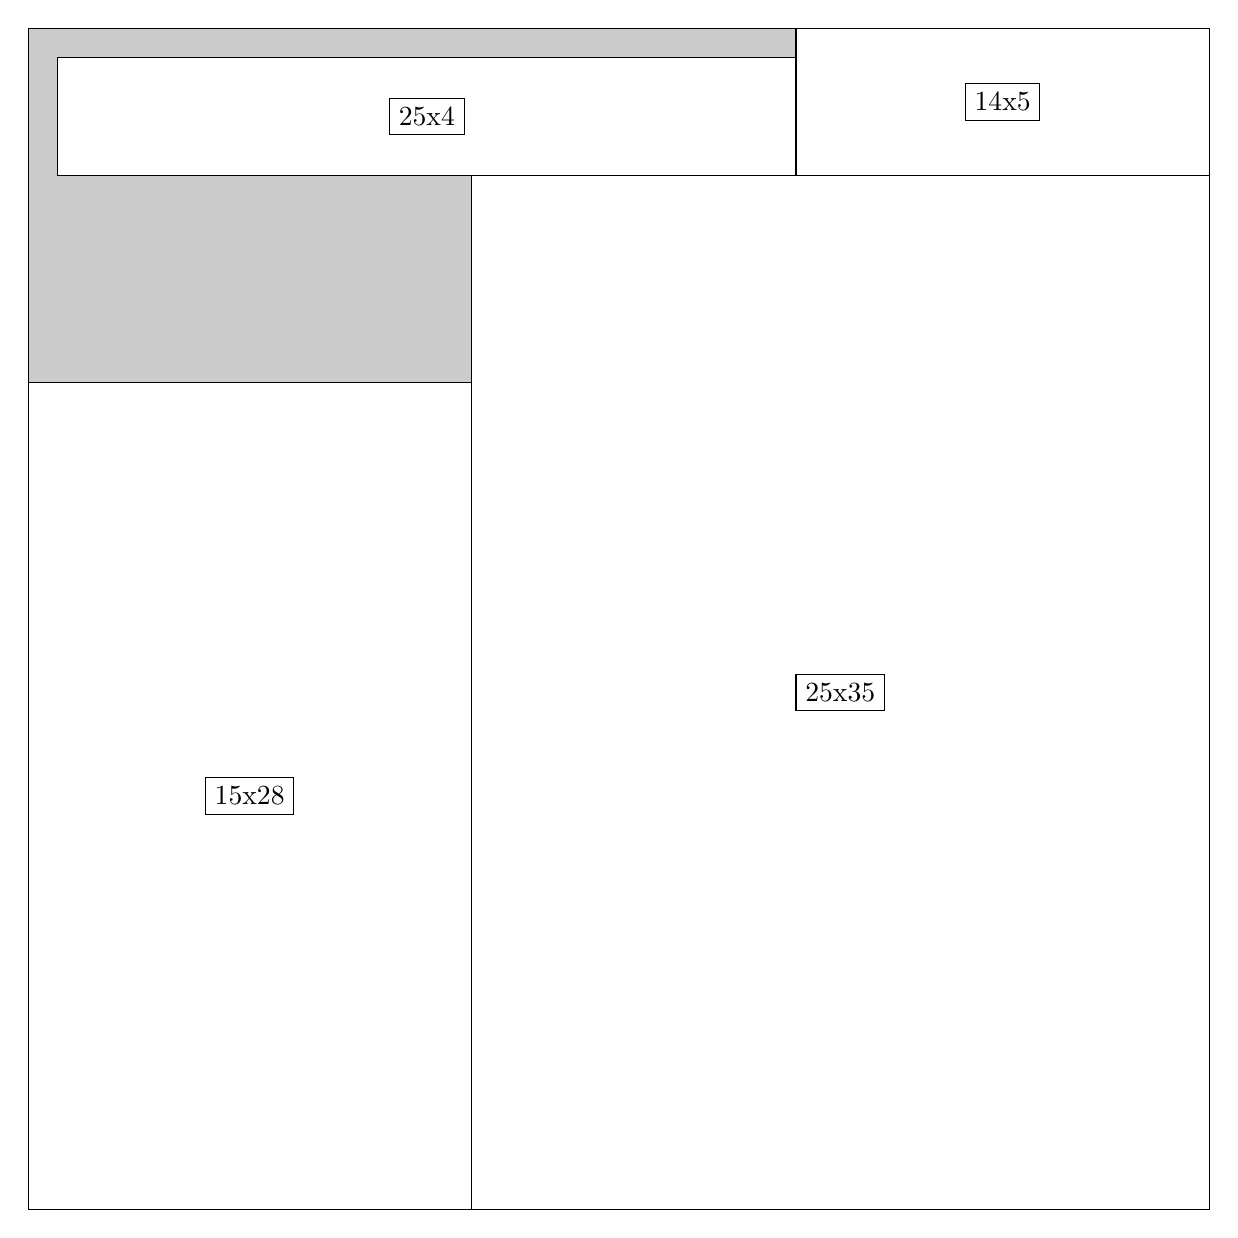
\begin{tikzpicture}[shorten >=1pt,scale=1.0,every node/.style={scale=1.0},->]
\tikzstyle{vertex}=[circle,fill=black!25,minimum size=14pt,inner sep=0pt]
\filldraw[fill=gray!40!white, draw=black] (0,0) rectangle (15.0,15.0);
\foreach \name/\x/\y/\w/\h in {25x35/5.625/0.0/9.375/13.125,15x28/0.0/0.0/5.625/10.5,14x5/9.75/13.125/5.25/1.875,25x4/0.375/13.125/9.375/1.5}
\filldraw[fill=white!40!white, draw=black] (\x,\y) rectangle node[draw] (\name) {\name} ++(\w,\h);
\end{tikzpicture}


w =25 , h =35 , x =15 , y =0 , v =875
\par
w =15 , h =28 , x =0 , y =0 , v =420
\par
w =14 , h =5 , x =26 , y =35 , v =70
\par
w =25 , h =4 , x =1 , y =35 , v =100
\par
\newpage


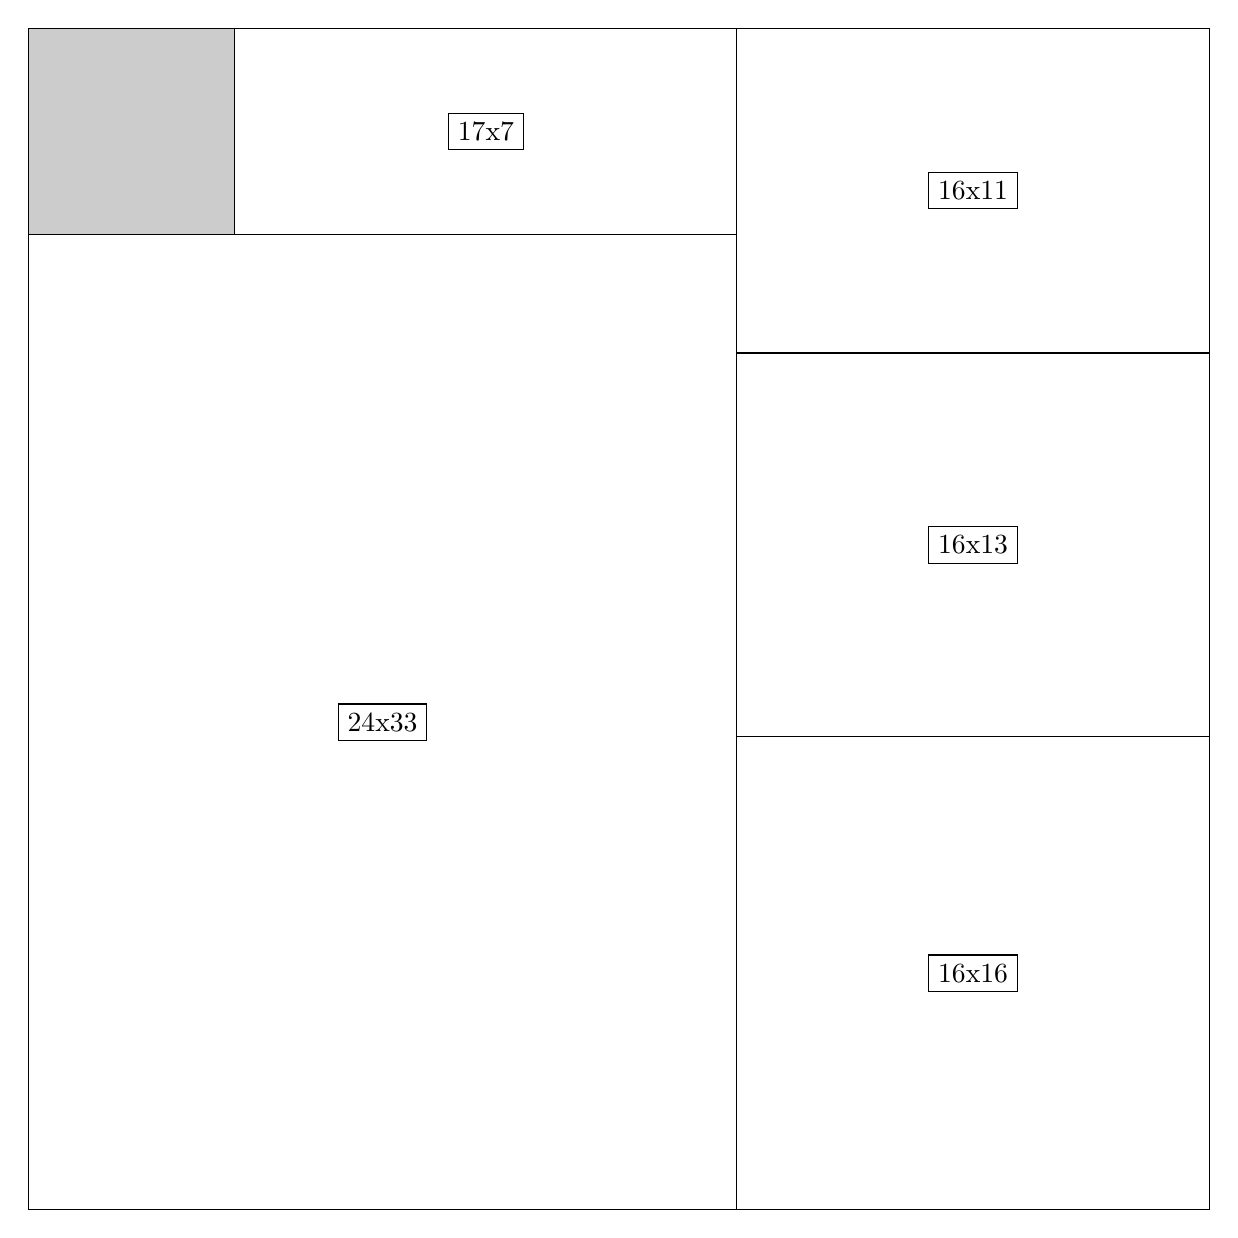
\begin{tikzpicture}[shorten >=1pt,scale=1.0,every node/.style={scale=1.0},->]
\tikzstyle{vertex}=[circle,fill=black!25,minimum size=14pt,inner sep=0pt]
\filldraw[fill=gray!40!white, draw=black] (0,0) rectangle (15.0,15.0);
\foreach \name/\x/\y/\w/\h in {16x16/9.0/0.0/6.0/6.0,16x13/9.0/6.0/6.0/4.875,16x11/9.0/10.875/6.0/4.125,24x33/0.0/0.0/9.0/12.375,17x7/2.625/12.375/6.375/2.625}
\filldraw[fill=white!40!white, draw=black] (\x,\y) rectangle node[draw] (\name) {\name} ++(\w,\h);
\end{tikzpicture}


w =16 , h =16 , x =24 , y =0 , v =256
\par
w =16 , h =13 , x =24 , y =16 , v =208
\par
w =16 , h =11 , x =24 , y =29 , v =176
\par
w =24 , h =33 , x =0 , y =0 , v =792
\par
w =17 , h =7 , x =7 , y =33 , v =119
\par
\newpage


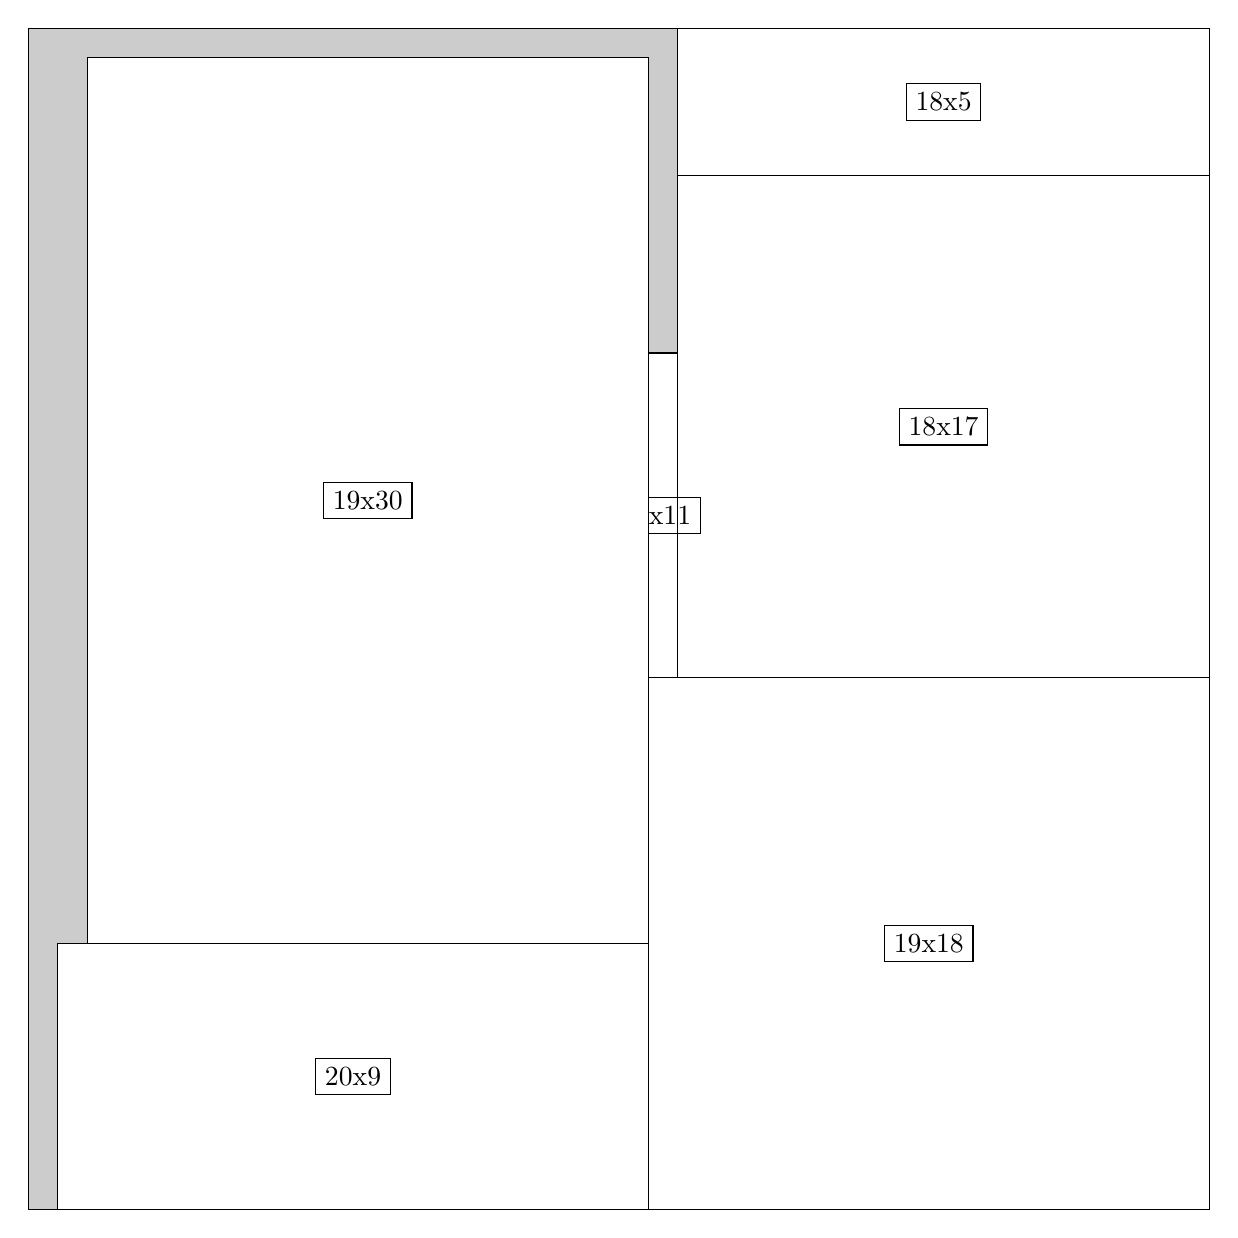
\begin{tikzpicture}[shorten >=1pt,scale=1.0,every node/.style={scale=1.0},->]
\tikzstyle{vertex}=[circle,fill=black!25,minimum size=14pt,inner sep=0pt]
\filldraw[fill=gray!40!white, draw=black] (0,0) rectangle (15.0,15.0);
\foreach \name/\x/\y/\w/\h in {19x18/7.875/0.0/7.125/6.75,18x17/8.25/6.75/6.75/6.375,1x11/7.875/6.75/0.375/4.125,18x5/8.25/13.125/6.75/1.875,20x9/0.375/0.0/7.5/3.375,19x30/0.75/3.375/7.125/11.25}
\filldraw[fill=white!40!white, draw=black] (\x,\y) rectangle node[draw] (\name) {\name} ++(\w,\h);
\end{tikzpicture}


w =19 , h =18 , x =21 , y =0 , v =342
\par
w =18 , h =17 , x =22 , y =18 , v =306
\par
w =1 , h =11 , x =21 , y =18 , v =11
\par
w =18 , h =5 , x =22 , y =35 , v =90
\par
w =20 , h =9 , x =1 , y =0 , v =180
\par
w =19 , h =30 , x =2 , y =9 , v =570
\par
\newpage


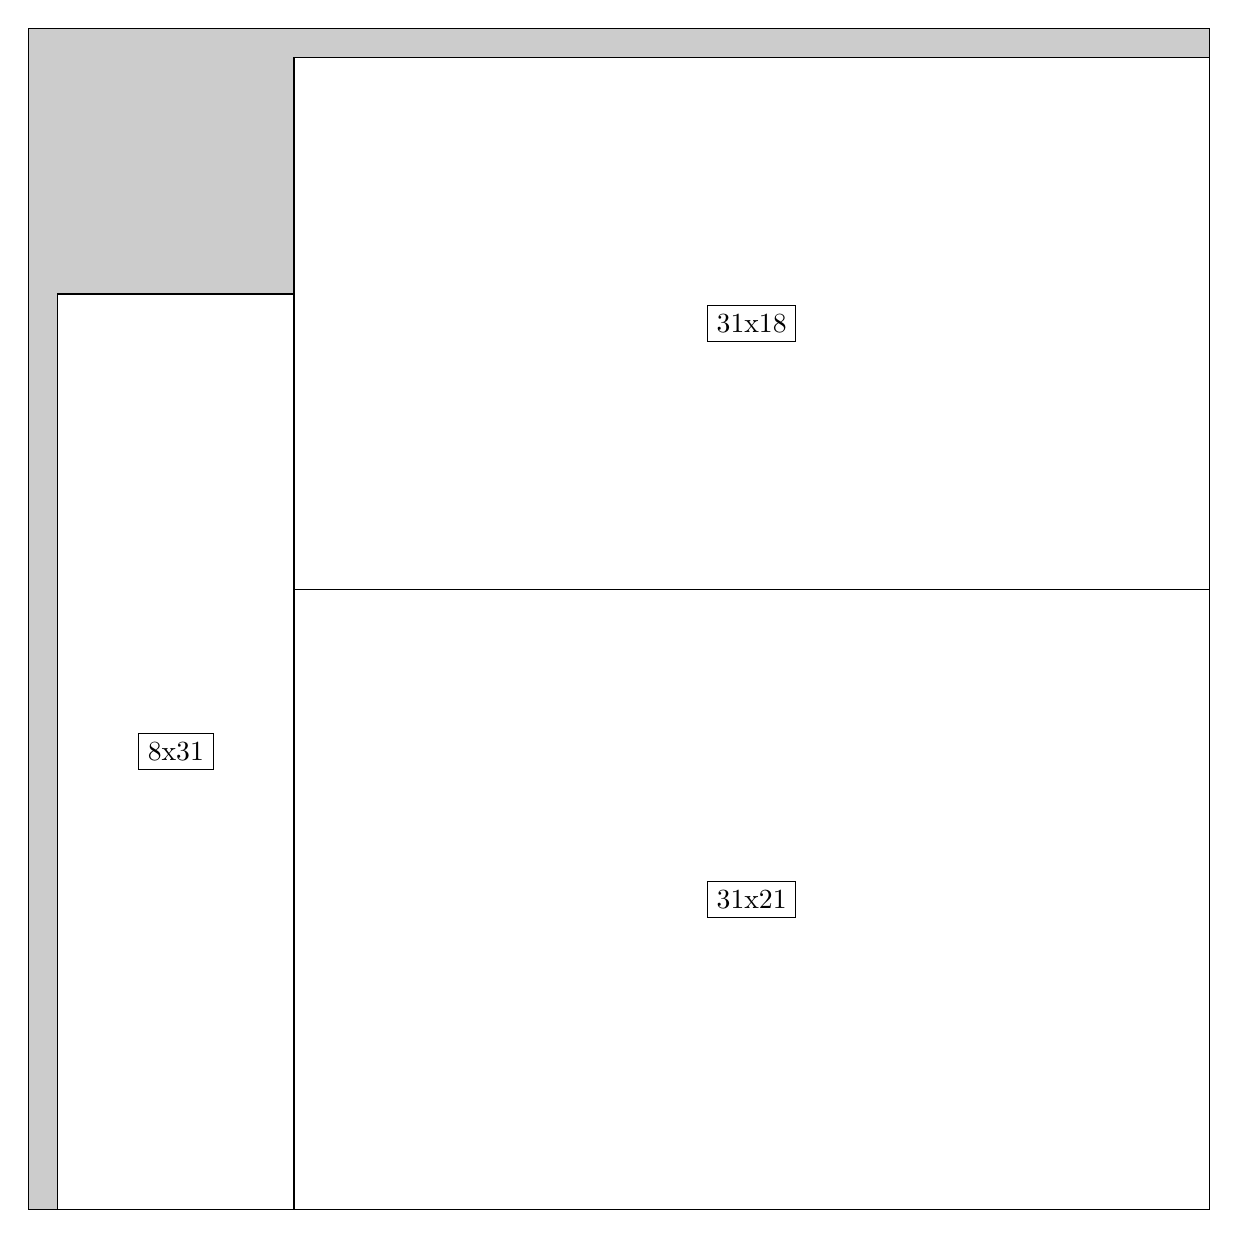
\begin{tikzpicture}[shorten >=1pt,scale=1.0,every node/.style={scale=1.0},->]
\tikzstyle{vertex}=[circle,fill=black!25,minimum size=14pt,inner sep=0pt]
\filldraw[fill=gray!40!white, draw=black] (0,0) rectangle (15.0,15.0);
\foreach \name/\x/\y/\w/\h in {31x21/3.375/0.0/11.625/7.875,31x18/3.375/7.875/11.625/6.75,8x31/0.375/0.0/3.0/11.625}
\filldraw[fill=white!40!white, draw=black] (\x,\y) rectangle node[draw] (\name) {\name} ++(\w,\h);
\end{tikzpicture}


w =31 , h =21 , x =9 , y =0 , v =651
\par
w =31 , h =18 , x =9 , y =21 , v =558
\par
w =8 , h =31 , x =1 , y =0 , v =248
\par
\newpage


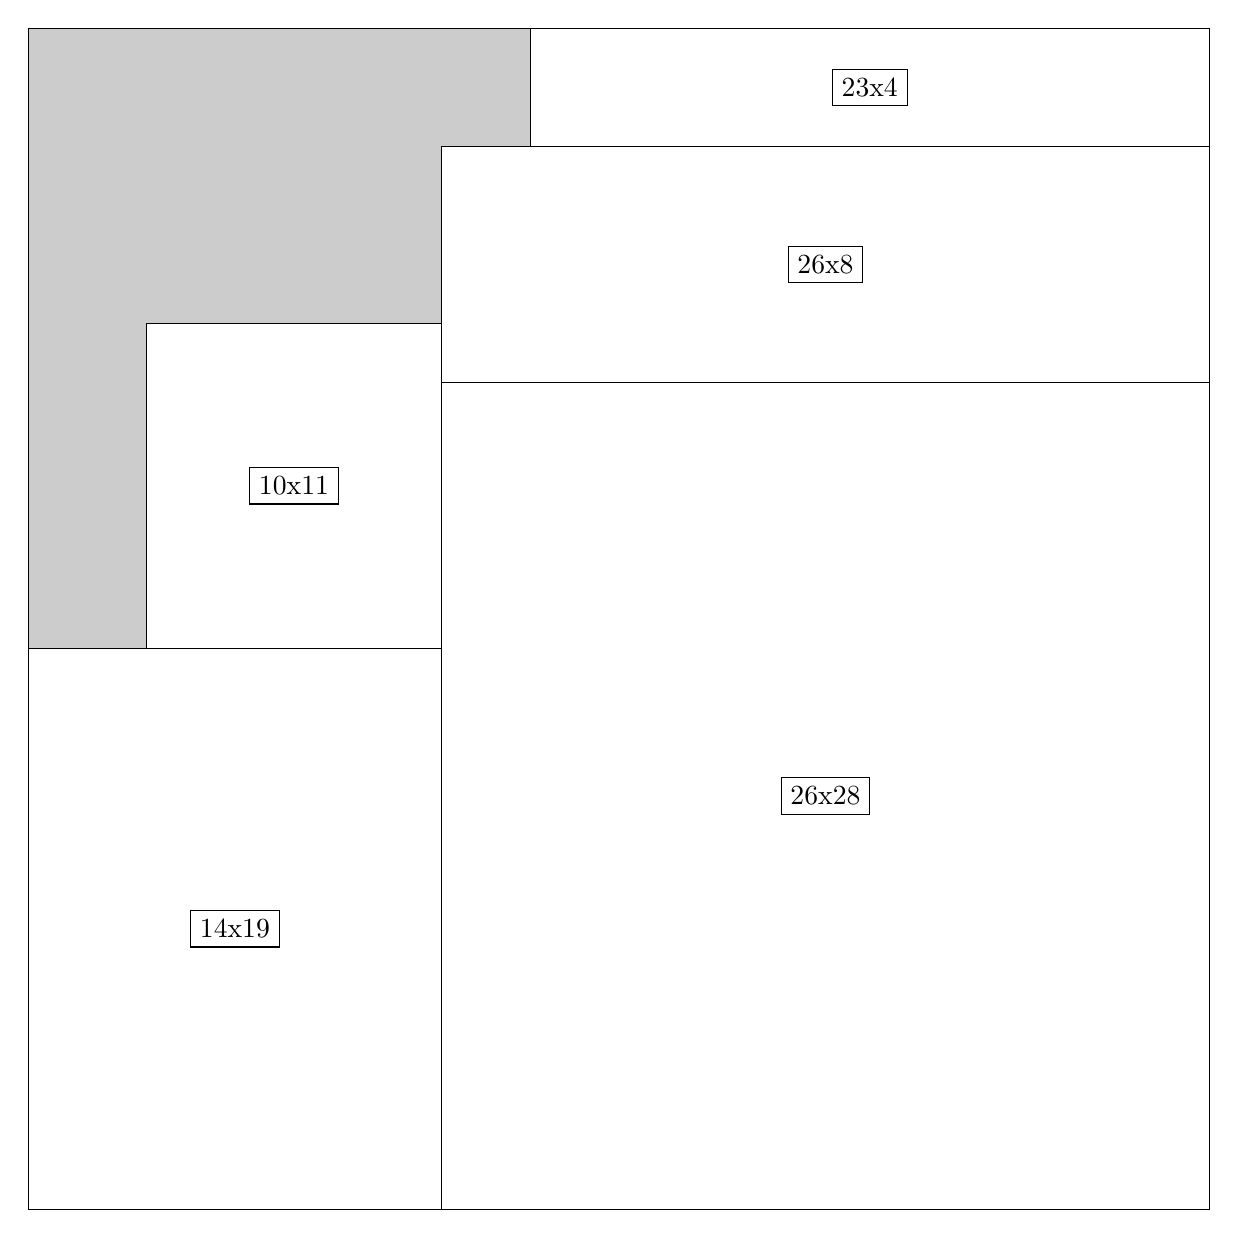
\begin{tikzpicture}[shorten >=1pt,scale=1.0,every node/.style={scale=1.0},->]
\tikzstyle{vertex}=[circle,fill=black!25,minimum size=14pt,inner sep=0pt]
\filldraw[fill=gray!40!white, draw=black] (0,0) rectangle (15.0,15.0);
\foreach \name/\x/\y/\w/\h in {26x28/5.25/0.0/9.75/10.5,26x8/5.25/10.5/9.75/3.0,23x4/6.375/13.5/8.625/1.5,14x19/0.0/0.0/5.25/7.125,10x11/1.5/7.125/3.75/4.125}
\filldraw[fill=white!40!white, draw=black] (\x,\y) rectangle node[draw] (\name) {\name} ++(\w,\h);
\end{tikzpicture}


w =26 , h =28 , x =14 , y =0 , v =728
\par
w =26 , h =8 , x =14 , y =28 , v =208
\par
w =23 , h =4 , x =17 , y =36 , v =92
\par
w =14 , h =19 , x =0 , y =0 , v =266
\par
w =10 , h =11 , x =4 , y =19 , v =110
\par
\newpage


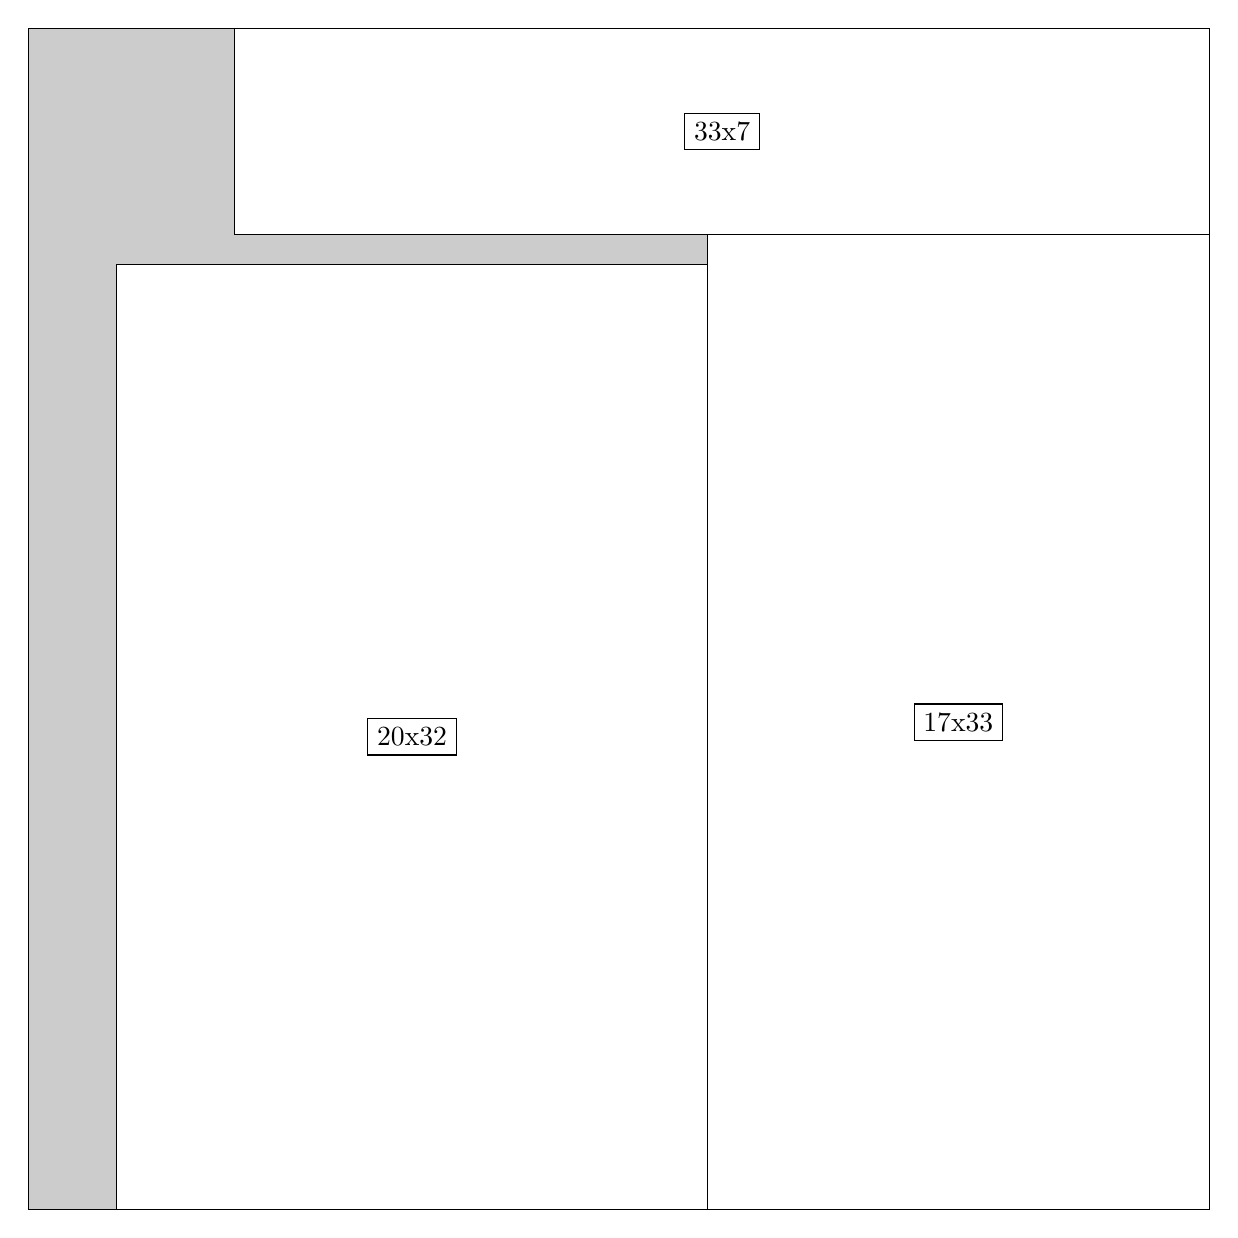
\begin{tikzpicture}[shorten >=1pt,scale=1.0,every node/.style={scale=1.0},->]
\tikzstyle{vertex}=[circle,fill=black!25,minimum size=14pt,inner sep=0pt]
\filldraw[fill=gray!40!white, draw=black] (0,0) rectangle (15.0,15.0);
\foreach \name/\x/\y/\w/\h in {17x33/8.625/0.0/6.375/12.375,20x32/1.125/0.0/7.5/12.0,33x7/2.625/12.375/12.375/2.625}
\filldraw[fill=white!40!white, draw=black] (\x,\y) rectangle node[draw] (\name) {\name} ++(\w,\h);
\end{tikzpicture}


w =17 , h =33 , x =23 , y =0 , v =561
\par
w =20 , h =32 , x =3 , y =0 , v =640
\par
w =33 , h =7 , x =7 , y =33 , v =231
\par
\newpage


\end{document}